\begin{center}
	\fbox{\textbf{Resolução da Lista 01}}
\end{center}
\begin{tcolorbox}[
	enhanced,
	sharp corners,
	boxrule=0.5pt,
	colback=white, 
	colframe=black,         
	width=1\textwidth,
	%fontupper=\itshape
	]%
	\textbf{Resumo:} Este documento apresenta a resolução detalhada da primeira lista de exercícios da disciplina de Variedades Diferenciáveis. O conteúdo aborda os fundamentos da topologia e da geometria diferencial, incluindo a construção de atlas suaves e maximais, a análise de conectividade em variedades, a estrutura de subvariedades suaves via Teorema do Valor Regular, a geometria de esferas ($\mathbb{S}^n$) e espaços projetivos ($\mathbb{RP}^n$), além de uma introdução formal aos Grupos de Lie e suas propriedades algébricas e topológicas.
\end{tcolorbox}
%%%% QUESTÃO 01 %%%%
\questao{
	Seja $M^{n}$ uma $n$-variedade topológica. Mostre que:
	\begin{enumerate}[label=(\alph*)]
		\item Qualquer atlas suave para $M^{n}$ está contido em um atlas suave maximal (único).
		\item Dois atlas suaves para $M^{n}$ determinam o mesmo atlas suave maximal se, e somente se, a união desses atlas é um atlas suave.
	\end{enumerate}
}
\solucao{
	
	\textbf{Análise do Enunciado}
	\begin{itemize}
		\item \textbf{Hipóteses:} $M^n$ é uma $n$-variedade topológica.
		\item \textbf{Tese (a):} Provar a existência e unicidade de um atlas suave maximal que contenha qualquer atlas suave dado.
		\item \textbf{Tese (b):} Caracterizar a equivalência de atlas suaves através da suavidade de sua união.
	\end{itemize}
	\vspace{5pt}
	\textbf{(a)} Seja $\mathcal{A} = \{(U_\alpha, \varphi_\alpha)\}_{\alpha \in \Lambda}$ um atlas suave para $M^n$. Definimos a coleção $\overline{\mathcal{A}}$ como o conjunto de todas as cartas coordenadas que são suavemente compatíveis com todas as cartas de $\mathcal{A}$:
	\[ \overline{\mathcal{A}} = \{ (V, \psi) : (V, \psi) \text{ é suavemente compatível com toda carta } (U_\alpha, \varphi_\alpha) \in \mathcal{A} \}. \]
	
	Claramente $\mathcal{A} \subseteq \overline{\mathcal{A}}$, pois as cartas de um atlas suave são, por definição, compatíveis entre si. Para mostrar que $\overline{\mathcal{A}}$ é um atlas suave, devemos provar que quaisquer duas cartas $(V_1, \psi_1), (V_2, \psi_2) \in \overline{\mathcal{A}}$ são suavemente compatíveis. 
	
	Seja $p \in V_1 \cap V_2$. Como $\mathcal{A}$ é um atlas, existe uma carta $(U_\alpha, \varphi_\alpha) \in \mathcal{A}$ tal que $p \in U_\alpha$. Definimos o aberto $W = V_1 \cap V_2 \cap U_\alpha$. A aplicação de transição $\psi_2 \circ \psi_1^{-1}$ restrita ao domínio $\psi_1(W) \subset \mathbb{R}^n$ pode ser fatorada como:
	\[ \psi_2 \circ \psi_1^{-1} \Big|_{\psi_1(W)} = \underbrace{(\psi_2 \circ \varphi_\alpha^{-1})}_{\text{suave}} \circ \underbrace{(\varphi_\alpha \circ \psi_1^{-1})}_{\text{suave}}. \]
	
	Visto que ambas as funções no lado direito são suaves (pela definição de $\overline{\mathcal{A}}$), a sua composição também é suave em uma vizinhança de $\psi_1(p)$. Como isso é válido para todo ponto na interseção, concluímos que $\overline{\mathcal{A}}$ é um atlas suave.
	
	\textbf{Maximalidade:} Para mostrar que $\overline{\mathcal{A}}$ é maximal, seja $(V, \psi)$ uma carta suave compatível com todas as cartas de $\overline{\mathcal{A}}$. Como $\mathcal{A} \subseteq \overline{\mathcal{A}}$, em particular, $(V, \psi)$ deve ser compatível com todas as cartas de $\mathcal{A}$. Por definição de $\overline{\mathcal{A}}$, qualquer carta compatível com $\mathcal{A}$ já pertence a $\overline{\mathcal{A}}$. Logo, $(V, \psi) \in \overline{\mathcal{A}}$, o que prova que $\overline{\mathcal{A}}$ é maximal.
	
	\textbf{Unicidade:} Suponha que exista outro atlas maximal $\mathcal{C}$ tal que $\mathcal{A} \subseteq \mathcal{C}$. Como $\mathcal{C}$ é um atlas suave, todas as suas cartas são mutuamente compatíveis. Como $\mathcal{A} \subseteq \mathcal{C}$, todas as cartas de $\mathcal{C}$ são compatíveis com todas as cartas de $\mathcal{A}$. Pela definição de $\overline{\mathcal{A}}$, isto implica $\mathcal{C} \subseteq \overline{\mathcal{A}}$. Por maximalidade de $\mathcal{C}$, temos $\mathcal{C} = \overline{\mathcal{A}}$.
	
	\textbf{(b)} $(\implies)$ Suponha que $\mathcal{A}$ e $\mathcal{B}$ determinam o mesmo atlas suave maximal $\mathcal{M}$. Por definição, $\mathcal{A} \subseteq \mathcal{M}$ e $\mathcal{B} \subseteq \mathcal{M}$. Logo, $\mathcal{A} \cup \mathcal{B} \subseteq \mathcal{M}$. Como subconjuntos de cartas de um atlas suave são mutuamente compatíveis, $\mathcal{A} \cup \mathcal{B}$ é um atlas suave.
	
	$(\impliedby)$ Suponha agora que $\mathcal{A} \cup \mathcal{B}$ seja um atlas suave. Seja $\mathcal{M}$ o atlas suave maximal único que contém a união $\mathcal{A} \cup \mathcal{B}$ (cuja existência foi garantida no item (a)). 
	
	Como $\mathcal{A} \subseteq (\mathcal{A} \cup \mathcal{B}) \subseteq \mathcal{M}$, então $\mathcal{M}$ é um atlas suave maximal que contém $\mathcal{A}$. Pela unicidade, $\mathcal{A}_{max} = \mathcal{M}$. Da mesma forma, como $\mathcal{B} \subseteq (\mathcal{A} \cup \mathcal{B}) \subseteq \mathcal{M}$, temos $\mathcal{B}_{max} = \mathcal{M}$. Portanto, $\mathcal{A}_{max} = \mathcal{B}_{max}$.
}
%%%% QUESTÃO 02 %%%%
\questao{
	Mostre que uma $n$-variedade suave $M^{n}$ é conexa se, e somente se, ela é conexa por caminhos.
}
\solucao{
	
	\textbf{Análise do Enunciado}
	\begin{itemize}
		\item \textbf{Hipóteses:} $M^n$ é uma $n$-variedade suave.
		\item \textbf{Tese:} Provar a equivalência entre a conexidade topológica e a conexidade por caminhos.
	\end{itemize}
	\vspace{5pt}
	\textbf{($\Leftarrow$)} Suponha que $M$ seja conexa por caminhos. Provaremos que $M$ é conexa por contradição. Se $M$ fosse desconexa, existiriam abertos $U, V \subset M$ não vazios e disjuntos tais que $M = U \cup V$. Sejam $p \in U$ e $q \in V$. Por hipótese, existe $\gamma: [0,1] \to M$ contínua com $\gamma(0) = p$ e $\gamma(1) = q$.
	
	Os conjuntos $A = \gamma^{-1}(U)$ e $B = \gamma^{-1}(V)$ seriam abertos em $[0,1]$ pela continuidade de $\gamma$. Teríamos $A \cup B = [0,1]$, $A \cap B = \emptyset$, com $0 \in A$ e $1 \in B$ (logo ambos não vazios). Isso contradiz a conexidade de $[0,1]$. Portanto, $M$ é conexa.
	
	\textbf{($\Rightarrow$)} Suponha $M$ conexa. Fixemos $p \in M$ e definamos o conjunto de pontos que podem ser ligados a $p$ por um caminho contínuo:
	\[ A = \{ q \in M : \exists \, \sigma: [0,1] \to M \text{ contínua com } \sigma(0)=p \text{ e } \sigma(1)=q \}. \]
	
	\textbf{1. $A$ é aberto:} Seja $q \in A$. Existe uma vizinhança coordenada $U$ de $q$ homeomorfa a uma bola em $\mathbb{R}^n$, a qual é conexa por caminhos. Seja $\phi: U \to B^n$ o homeomorfismo. Para qualquer $q' \in U$, definimos o caminho interno $\alpha: [0,1] \to U$ por $\alpha(t) = \phi^{-1}\left((1-t)\phi(q) + t\phi(q')\right)$. Como $q \in A$, existe $\sigma: [0,1] \to M$ de $p$ a $q$. Definimos a concatenação $\beta: [0,1] \to M$:
	\[ \beta(t) = \begin{cases} \sigma(2t), & 0 \leq t \leq 1/2 \\ \alpha(2t-1), & 1/2 < t \leq 1 \end{cases} \]
	$\beta$ é contínua pelo Lema da Colagem ($\sigma(1)=q=\alpha(0)$) e liga $p$ a $q'$. Logo $U \subseteq A$, e $A$ é aberto.
	
	\textbf{2. $A$ é fechado:} Seja $r \in \overline{A}$. Seja $V$ uma vizinhança coordenada de $r$ (homeomorfa a uma bola). Pela definição de fecho, existe $s \in V \cap A$. Como $s \in A$, ele se liga a $p$. Como $s$ e $r$ estão na mesma vizinhança conexa por caminhos $V$, eles se ligam. Por concatenação, $r \in A$. Logo $\overline{A} = A$.
	
	Como $M$ é conexo e $A$ é aberto, fechado e não vazio, $A = M$.
}
%%%% QUESTÃO 03 %%%%
\questao{
	Seja $\mathbb{S}^{n}=\{(x^{1},...,x^{n+1})\in\mathbb{R}^{n+1}; (x^{1})^{2}+\dots+(x^{n+1})^{2}=1\}$ a esfera unitária. Prove que:
	\begin{enumerate}[label=(\alph*)]
		\item $\mathbb{S}^{n}$ é uma $n$-variedade suave, compacta e de Hausdorff com base enumerável exibindo um atlas suave sobre $\mathbb{S}^{n}$.
		\item $\mathbb{S}^{n}$ é a imagem inversa de um valor regular de uma função apropriada.
		\item Mostre que existe um atlas suave de $\mathbb{S}^{n}$ com apenas duas cartas.
		\item $\hat{E}$ possível obtermos um atlas suave para $\mathbb{S}^{n}$ com apenas uma carta?
	\end{enumerate}
}
\solucao{
	
	\textbf{Análise do Enunciado}
	\begin{itemize}
		\item \textbf{Hipóteses:} $\mathbb{S}^n$ definida como a esfera unitária em $\mathbb{R}^{n+1}$.
		\item \textbf{Tese (a):} Provar que $\mathbb{S}^n$ é uma $n$-variedade suave, compacta, Hausdorff e com base enumerável.
		\item \textbf{Tese (b):} Representar $\mathbb{S}^n$ como $f^{-1}(c)$ com $c$ valor regular.
		\item \textbf{Tese (c):} Construir um atlas de duas cartas.
		\item \textbf{Tese (d):} Provar a impossibilidade de um atlas de uma única carta.
	\end{itemize}
	\vspace{5pt}
	\textbf{(a)} Como $\mathbb{S}^n \subset \mathbb{R}^{n+1}$, então pela topologia induzida ela herda as propriedades de \textbf{Hausdorff} e \textbf{base enumerável}. 
	
	\textbf{1. Compacidade}
	
	Seja $f: \mathbb{R}^{n+1} \to \mathbb{R}$ dada por $f(x) = |x|^2$. Como $f$ é contínua e $\mathbb{S}^n = f^{-1}(1)$, a esfera é um conjunto fechado. Sendo também limitada ($|x|=1$), pelo Teorema de Heine-Borel, $\mathbb{S}^n$ é compacta.
	
	\textbf{2. Construção do Atlas das Calotas Polares}
	
	Para cada $i\in\{1,\ldots,n+1\}$, definimos os abertos $U_i^{\pm} = \{x \in \mathbb{S}^n : \pm x^i > 0\}$ e 
	\begin{eqnarray*}
		\varphi_i^{\pm}: U_i^{\pm}&\longrightarrow &\mathbb{R}^n\\
		(x^1, \dots,x^{n+1})&\longmapsto& (x^1, \dots, \widehat{x^i}, \dots, x^{n+1})
	\end{eqnarray*}
	onde, $\widehat{x^i}$ denota que $x_i$ é omitido.
	
	\textbf{Prova de Cobertura}: Seja $x = (x^1, \dots, x^{n+1}) \in \mathbb{S}^n$. Como $|x|^2 = 1$, é impossível que todas as coordenadas de $x$ sejam nulas. Portanto, existe pelo menos um $i \in \{1, \dots, n+1\}$ tal que $x^i \neq 0$. Se $x^i > 0$, então $x \in U_i^+$; se $x^i < 0$, então $x \in U_i^-$.	Isso implica que $\mathbb{S}^n = \bigcup_{i=1}^{n+1} (U_i^+ \cup U_i^-)$.
	
	Notemos que $\varphi_i^{\pm}$ são contínuas e além disso, $\varphi_i^{\pm}( U_i^{\pm})=\mathbb{B}^n$, onde $\mathbb{B}^n=\{x\in\mathbb{R}^n;|x|<1\}$. De fato, dado $x\in U_i^{\pm}$, temos que:
	$$|\varphi_i^{\pm}(x)|^2=(x^1)^2+\cdots+(x^{i-1})^2+(x^{i+1})^2+\cdots+(x^n)^2<(x^1)^2+\cdots+(x^{i-1})^2+(x^i)^2+(x^{i+1})^2+\cdots+(x^n)^2=1.$$ 
	
	\textbf{Cálculo da Inversa}: A inversa $(\varphi_i^{\pm})^{-1}: \mathbb{B}^n\rightarrow U_i^{\pm}$, é obtida isolando $x^i$:
	$$(x^i)^2 = 1 - \sum_{k \neq i} (x^k)^2 \implies x^i = \pm \sqrt{1 - |u|^2},$$ 
	donde
	$$(\varphi_i^{\pm})^{-1}(u)=(u^1, \dots, u^{i-1},\pm\sqrt{1-|u|^2}, u^{i+1}, \dots, u^n),$$ que também são contínuas.
	
	Além disso, temos que $(\varphi_i^{\pm})^{-1}(\mathbb{B}^n)=U_i^{\pm}$, pois
	$$|(\varphi_i^{\pm})^{-1}(u)|^2=(u^1)^2+\cdots+(u^{i-1})^2+1-|u|^2+(u^{i+1})^2+\cdots(u^n)^2=1.$$
	
	Assim, cada uma das $2(n+1)$ cartas $\varphi_i^{\pm}$ é um homeomorfismo de $U_i^{\pm}$ sobre o aberto $\mathbb{B}^n \subset \mathbb{R}^n$, donde $\{(U_i^{\pm}, \varphi_i^{\pm})\}$ constitui um atlas topológico para $\mathbb{S}^n$. Portanto, $\mathbb{S}^n$ é uma $n$-variedade topológica.
	
	\textbf{3. Suavidade das Transições}
	
	A transição $\psi = \varphi_j^{\pm} \circ (\varphi_i^{\pm})^{-1}$ (para $i < j$) em $u \in \varphi_i^+(U_i^+ \cap U_j^+)\subset\mathbb{B}^n$ resulta em:
	$$ \psi(u) = (u^1, \dots, \pm\sqrt{1-|u|^2}, \dots, \widehat{u^j}, \dots, u^n) $$
	Como $|u|^2 < 1$, então a raiz quadrada é suave em $(0, \infty)$, e portanto a transição é suave. De forma similar, vale quando $i>j$. Quando $i=j$, então $\varphi_j^{\pm}\circ(\varphi_i^{\pm})^{-1}=\operatorname{Id}_{\mathbb{B}^n}$ que é suave.
	
	Concluímos que, $\{U_i^{\pm},\varphi_i^{\pm}\}$ é um atlas suave para $\mathbb{S}^n$, e portanto a esfera é uma $n$-variedade suave com essa estrutura.
	
	\textbf{(b)} Consideremos a função diferenciável,
	\begin{eqnarray*}
		f: \mathbb{R}^{n+1}&\longrightarrow &\mathbb{R}\\
		x&\longmapsto& f(x)=\langle x,x\rangle=|x|^2.
	\end{eqnarray*}
	Temos que $\nabla f(x) = 2x$ que é não nulo para todo $x\neq \vec{0}$. Em particular, $1$ é valor regular de $f$, donde $\mathbb{S}^n=f^{-1}(1)$.
	
	\textbf{(c)} Exibiremos o atlas de duas cartas via Projeção Estereográfica. Sejam $U_N = \mathbb{S}^n \setminus \{N\}$ e $U_S = \mathbb{S}^n \setminus \{S\}$, onde $N = (0,\dots,1)$ e $S = (0,\dots,-1)$. Notemos que, $\mathbb{S}^n=U_N\cup U_S$, ou seja, temos uma cobertura.
	
	\textbf{1. Dedução Geométrica e Construção do Atlas Suave}
	
	Para qualquer ponto $x = (x^1, \dots, x^{n+1}) \in U_N$, a projeção estereográfica $\phi_N(x)$ é definida como a interseção da semirreta que parte de $N$ e passa por $x$ com o hiperplano $x_{n+1}=0$ (identificado com $\mathbb{R}^n$).		
	
	A parametrização da reta $Nx$ é dada por $L(t) = N + t(x - N) = (0, \dots, 0, 1) + t(x^1, \dots, x^n, x^{n+1}-1)$ e ela intercepta o hiperplano $x_{n+1}=0$ se, e somente se:
	$$1 + t(x^{n+1} - 1) = 0 \implies t = \frac{1}{1 - x^{n+1}}.$$
	
	\begin{figure}[htbp]
		\centering
		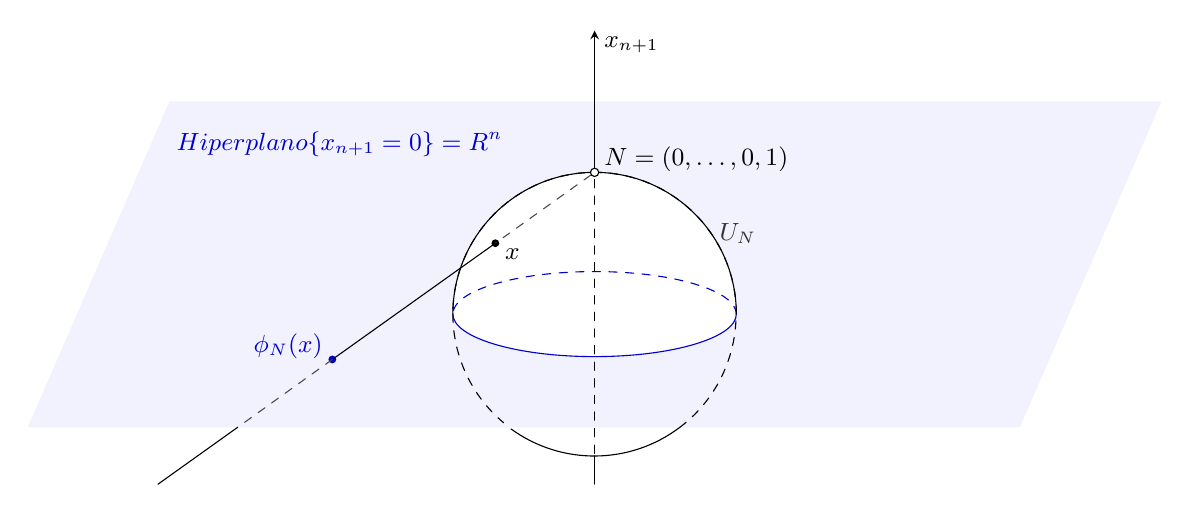
\begin{tikzpicture}[scale=1.8, line join=round, line cap=round]
			% --- Configurações de Estilo ---
			\tikzset{
				projection_inside/.style={thin, dashed, black!70}, 
				projection_outside/.style={thin, black}, 
				sphere_line/.style={thin, black},
				plane_line/.style={thin, blue!40!black}, 
				point/.style={circle, fill=black, inner sep=1pt},
				open_point/.style={circle, draw=black, fill=white, inner sep=0pt, minimum size=3pt},
				color_Int/.style={blue!80!black},
				color_Plane_Fill/.style={fill=blue!5, draw=none} 
			}
			
			% --- 1. O Plano R^n ---
			\fill[color_Plane_Fill] (-4, -0.8) -- (3, -0.8) -- (4, 1.5) -- (-3, 1.5) -- cycle;
			
			% Máscara para limpar o interior da esfera (apenas topo e equador)
			\fill[white] (1,0) arc (0:180:1) arc (180:360:1 and 0.3) -- cycle;
			
			% Rótulo R^n
			\node[color_Int, font=\small] at (-1.8,1.2) {$\text{Hiperplano } \{x_{n+1}=0\}=\mathbb{R}^n$};
			
			% --- 2. A Esfera S^n ---
			% Borda Superior sólida
			\draw[sphere_line] (1,0) arc (0:180:1); 
			
			% Equador (Interseção) em AZUL
			\draw[color_Int, thin] (1,0) arc (0:-180:1 and 0.3); % Frente
			\draw[color_Int, dashed, thin] (1,0) arc (0:180:1 and 0.3); % Atrás
			
			% BORDA INFERIOR DINÂMICA:
			% Parte 1: Tracejada (dentro do plano) de 180° até approx 243° (y = -0.8)
			\draw[dashed, sphere_line] (1,0) arc (0:180:1); % Apenas para referência, ignorar
			\draw[dashed, sphere_line] (-1,0) arc (180:230:1); 
			% Parte 2: SÓLIDA (fora do plano) de 243° até 307° (y = -0.8)
			\draw[sphere_line] (0.6, -0.8) arc (307:234:1); % Ajustado para a base
			% Correção manual do arco inferior para precisão visual:
			%\draw[sphere_line] (-0.6, -0.8) arc (243:307:1);
			% Parte 3: Tracejada (dentro do plano) de 307° até 360°
			\draw[dashed, sphere_line] (0.6, -0.8) arc (307:360:1);
			
			% --- 3. Polos ---
			\node[open_point, label={[font=\small, above right, yshift=-5pt]:$N=(0,\ldots,0,1)$}] (N) at (0,1) {};
			
			% --- 4. Eixo x_{n+1} ---
			\draw[sphere_line, -{stealth}] (0, 1.03) -- (0, 2);       % Sólido superior
			\draw[dashed, sphere_line] (0, 0.95) -- (0, -1);       % Tracejado dentro da esfera
			\draw[sphere_line] (0, -1) -- (0, -1.2);            % Sólido ao sair do plano
			\node[right, font=\small] at (0, 1.9) {$x_{n+1}$};
			
			% --- 5. Geometria da Projeção ---
			\coordinate (P_new) at (-0.7, 0.5);
			\node[point, label={[font=\small, below right]:$x$}] at (P_new) {};
			
			% Ponto phi_N(x)
			\coordinate (U) at (-1.85, -0.32); 
			\node[point, color_Int, label={[font=\small, color=blue!80!black, above left, yshift=-5pt]:$\phi_N(x)$}] at (U) {};
			
			% Reta terminando em y = -1.2
			\coordinate (End) at (-3.08, -1.2);
			
			% Reta: 
			\draw[projection_inside] (N) -- (P_new); 
			\draw[projection_outside] (P_new) -- (U); 
			
			% Divisão da última parte:
			% 1. De phi_N(x) até a borda inferior do plano (-2.52, -0.8) -> Tracejado
			\draw[projection_inside] (U) -- (-2.52, -0.8); 
			% 2. Da borda do plano até o ponto final (End) -> Sólido
			\draw[projection_outside] (-2.52, -0.8) -- (End); 
			
			% --- 6. Rótulos dos Abertos ---
			\node[black!80, font=\small, xshift=-2pt] at (1.05, 0.57) {$U_N$};
		\end{tikzpicture}
		\caption{Projeção Estereográfica a partir do polo norte}
	\end{figure}
	
	Substituindo $t$ nas primeiras $n$ coordenadas de $L(t)$, obtemos a aplicação $\phi_N: U_N \to \mathbb{R}^n$:
	$$\boxed{\phi_N(x^1, \dots, x^{n+1}) = \left( \frac{x^1}{1-x^{n+1}}, \dots, \frac{x^n}{1-x^{n+1}} \right)},$$ que é contínua, pois é uma função racional cujas componentes são contínuas (o denominador $1-x^{n+1}\neq 0$ em $U_N$).
	
	De forma análoga, para $x \in U_S$, a reta $L_S(t) = S + t(x-S) = (0,\dots,-1) + t(x^1, \dots, x^{n+1}+1)$ intercepta $x_{n+1}=0$ quando $$-1+t(x^{n+1}+1)=0 \implies t = \frac{1}{1+x^{n+1}}.$$ 
	Assim, $\phi_S: U_S \to \mathbb{R}^n$ é dada por:
	$$\boxed{\phi_S(x) = \left( \frac{x^1}{1+x^{n+1}}, \dots, \frac{x^n}{1+x^{n+1}} \right),}$$ que é contínua, pois é uma função racional cujas componentes são contínuas (o denominador $1+x^{n+1}\neq 0$ em $U_S$).
	
	Além disso, notemos que $\phi_S(x)=-\phi_N(-x)$. 
	
	\textbf{Cálculo da Inversa $\phi_N^{-1}$}: Seja $u \in \mathbb{R}^n$, queremos $x \in U_N$ tal que $u^i = \frac{x^i}{1-x^{n+1}}$, ou seja, 
	$$\boxed{x^i = u^i(1-x^{n+1}).}\quad (\ast)$$ 
	Elevando ao quadrado e somando de $i=1$ até $n$:
	$$\sum_{i=1}^n (x^i)^2 = \sum_{i=1}^n [u^i(1-x^{n+1})]^2 = (1-x^{n+1})^2 \sum_{i=1}^n (u^i)^2 = |u|^2 (1-x^{n+1})^2$$
	Como $x \in U_N$, temos $\sum_{i=1}^n (x^i)^2 = 1 - (x^{n+1})^2$. Igualando as expressões:
	\begin{align*}
		1 - (x^{n+1})^2 &= |u|^2 (1-x^{n+1})^2 \\
		(1-x^{n+1})(1+x^{n+1}) &= |u|^2 (1-x^{n+1})^2 \\
		1+x^{n+1} &= |u|^2 (1-x^{n+1}) \quad (\text{pois } x \in U_N \implies x^{n+1} \neq 1) \\
		x^{n+1}(1+|u|^2) &= |u|^2 - 1 \implies x^{n+1} = \frac{|u|^2-1}{|u|^2+1}
	\end{align*}
	Substituindo $x^{n+1}$  em $(\ast)$, obtemos que: $$x^i = u^i \left(1 - \frac{|u|^2-1}{|u|^2+1}\right) = u^i \left(\frac{|u|^2+1 - |u|^2 + 1}{|u|^2+1}\right) = \frac{2u^i}{|u|^2+1}.$$
	
	Logo, $\phi_N^{-1}:\mathbb{R}^n\setminus\{0\}\rightarrow U_N$ é dada por:
	$$\phi_N^{-1}(u)=\frac{\left(2u^1,\dots,2u^n,|u|^2-1\right)}{|u|^2+1}$$
	
	\textbf{2. Suavidade das Transições}
	
	A transição $\psi = \phi_S \circ \phi_N^{-1}$ é definida no domínio $\phi_N(U_N \cap U_S) = \mathbb{R}\setminus\{0\}$. Além disso,
	\begin{align*}
		\psi^i(u) = \frac{x^i}{1+x^{n+1}} = \frac{\frac{2u^i}{|u|^2+1}}{1 + \frac{|u|^2-1}{|u|^2+1}} = \frac{2u^i}{|u|^2+1+|u|^2-1} = \frac{2u^i}{2|u|^2} = \frac{u^i}{|u|^2}
	\end{align*}
	A expressão $\psi(u) = \frac{u}{|u|^2}$ é suave em $\mathbb{R}^n \setminus \{0\}$, concluindo que o atlas $\{(U_N,\phi_N),(U_S,\phi_S)\}$ é suave. Portanto, $\mathbb{S}^n$ é uma $n$-variedade com essa estrutura.
	
	\textbf{(d)} Não é possível. Se existisse uma única carta $\phi: \mathbb{S}^n \to \mathbb{R}^n$, ela seria um homeomorfismo sobre um aberto $V \subseteq \mathbb{R}^n$. Pelo item (a), $\mathbb{S}^n$ é compacto, logo $V$ deveria ser um subconjunto compacto e aberto de $\mathbb{R}^n$. Como $\mathbb{R}^n$ é conexo, o único aberto e fechado (compacto) é o conjunto vazio ou o próprio $\mathbb{R}^n$ (que não é compacto). Como $\mathbb{S}^n \neq \emptyset$, chegamos a uma contradição.
}
%%%% QUESTÃO 04 %%%%
\questao{Mostre que o espaço projetivo real $\mathbb{RP}^n$ é uma $n$-variedade suave, compacta e de Hausdorff com base enumerável exibindo um atlas suave sobre $\mathbb{RP}^n$.
}
\solucao{
	
	\textbf{Análise do Enunciado}
	\begin{itemize}
		\item \textbf{Hipóteses:} $\mathbb{RP}^n$ definido como o espaço quociente de $\mathbb{R}^{n+1} \setminus \{0\}$ por $x \sim \lambda x$.
		\item \textbf{Tese:} Provar que $\mathbb{RP}^n$ é uma $n$-variedade suave, compacta, Hausdorff e com base enumerável.
	\end{itemize}
	\vspace{5pt}
	Definimos o espaço projetivo real $\mathbb{RP}^n$ como o espaço quociente de $\mathbb{R}^{n+1} \setminus \{0\}$ pela relação de equivalência $\sim$, onde $x \sim y$ se e somente se $y = \lambda x$ para algum $\lambda \in \mathbb{R} \setminus \{0\}$. Denotamos por $[x]$ a classe de equivalência de $x$.
	
	Consideremos a esfera unitária $\mathbb{S}^n \subset \mathbb{R}^{n+1}$. Definimos a aplicação de projeção canônica $\pi: \mathbb{S}^n \to \mathbb{RP}^n$ por $\pi(x) = [x]$. 
	
	\textbf{Sobrejetividade de $\pi$:} 
	
	Seja $[v] \in \mathbb{RP}^n$ com $v \in \mathbb{R}^{n+1} \setminus \{0\}$ e consideremos o ponto $x = \frac{v}{|v|} \in \mathbb{S}^n$. Como $v = |v|x$ e $|v| \neq 0$, temos que $v \sim x$, donde $\pi(x) = [x] = [v]$. Isso prova que $\pi$ é sobrejetiva. Como a relação $\sim$ em $\mathbb{S}^n$ reduz-se a $x \sim -x$, identificamos $\mathbb{RP}^n$ com o quociente $\mathbb{S}^n / \{x \sim -x\}$.
	
	\textbf{1. Compacidade}
	
	Como provamos na \textbf{Questão 3(a)}, $\mathbb{S}^n$ é compacta e sendo e $\pi$ contínua e sobrejetiva, $\mathbb{RP}^n = \pi(\mathbb{S}^n)$ é a imagem contínua de um compacto, e portanto, compacta.
	
	\textbf{2. Hausdorff e Base Enumerável}
	
	Sabemos que, se $X$ é um espaço compacto Hausdorff e a relação de equivalência $R \subset X \times X$ é um conjunto fechado, então o espaço quociente $X/R$ é Hausdorff. Aqui, $X = \mathbb{S}^n$ e $R = \{(x, -x) : x \in \mathbb{S}^n\}$. A aplicação $\alpha: \mathbb{S}^n \times \mathbb{S}^n \to \mathbb{R}^{n+1}$ dada por $\alpha(x,y) = x+y$ é contínua, e $R = \alpha^{-1}(\{0\})$. Como $\{0\}$ é fechado em $\mathbb{R}^{n+1}$, $R$ é fechado em $\mathbb{S}^n \times \mathbb{S}^n$. Logo, $\mathbb{RP}^n$ é Hausdorff. 
	
	A base enumerável é herdada de $\mathbb{S}^n$ via a aplicação de quociente aberta $\pi$.
	
	\textbf{3. Construção do Atlas Suave}
	
	Para cada $i \in \{1, \dots, n+1\}$, definimos os abertos $V_i = \{ x \in \mathbb{S}^n : x^i \neq 0 \}$. Sejam $U_i = \pi(V_i) \subset \mathbb{RP}^n$. 
	
	\textbf{Prova de Cobertura:} 
	
	Seja $[x] \in \mathbb{RP}^n$. Tomando um representante $x \in \mathbb{S}^n$, temos que $\sum_{j=1}^{n+1} (x^j)^2 = 1$. Isso implica que é impossível que todas as coordenadas $x^j$ sejam nulas simultaneamente. Logo, existe ao menos um índice $i \in \{1, \dots, n+1\}$ tal que $x^i \neq 0$. Assim, $x \in V_i$, o que implica $[x] \in \pi(V_i) = U_i$. Portanto, $\mathbb{RP}^n = \bigcup_{i=1}^{n+1} U_i$.
	
	Definimos as cartas $\phi_i: U_i \to \mathbb{R}^n$ por:
	$$ \boxed{\phi_i([x]) = \left( \frac{x^1}{x^i}, \dots, \frac{x^{i-1}}{x^i}, \frac{x^{i+1}}{x^i}, \dots, \frac{x^{n+1}}{x^i} \right).}$$
	\begin{figure}[htbp]
		\centering
		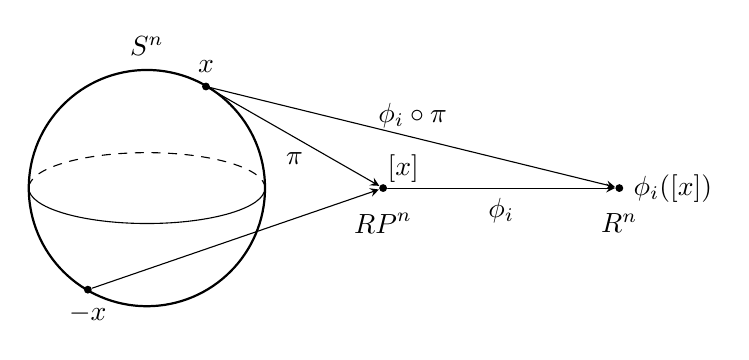
\begin{tikzpicture}[scale=1.5, line join=round, line cap=round]
			\tikzset{
				point/.style={circle, fill=black, inner sep=1pt},
				arrow/.style={->, >=stealth, thin}
			}
			% Esfera
			\draw[thick] (0,0) circle (1);
			\draw[dashed] (1,0) arc (0:180:1 and 0.3);
			\draw (1,0) arc (0:-180:1 and 0.3);
			
			% Pontos em S^n
			\node[point, label={above:$x$}] (X) at (0.5, 0.86) {};
			\node[point, label={below:$-x$}] (mX) at (-0.5, -0.86) {};
			
			% Espaço RP^n
			\node[point, label={right, xshift=-3.5pt, yshift=7pt:$[x]$}] (Proj) at (2, 0) {};
			
			% Espaço R^n
			\node[point, label={right:$\phi_i([x])$}] (R) at (4, 0) {};
			
			% Setas
			\draw[arrow] (X) -- (Proj) node[midway, below, yshift=-2pt] {$\pi$};
			\draw[arrow] (mX) -- (Proj);
			\draw[arrow] (Proj) -- (R) node[midway, below] {$\phi_i$};
			\draw[arrow] (X) -- (R) node[midway, above] {$\phi_i \circ \pi$};
			
			\node at (0, 1.2) {$\mathbb{S}^n$};
			\node at (2, -0.3) {$\mathbb{RP}^n$};
			\node at (4, -0.3) {$\mathbb{R}^n$};
		\end{tikzpicture}
		\caption{Diagrama de construção dos Atlas $\phi_i$}
	\end{figure}
	
	\textbf{Prova de Boa Definição:} 
	
	Para que $\phi_i$ seja bem definida, deve ter $\phi_i([x]) = \phi_i([y])$ sempre que $[x] = [y]$. Se $[x] = [y]$, então $y = \lambda x$ para algum $\lambda \neq 0$. Então:
	$$ \phi_i([y]) = \left( \frac{\lambda x^1}{\lambda x^i}, \dots, \frac{\lambda x^{n+1}}{\lambda x^i} \right) = \left( \frac{x^1}{x^i}, \dots, \frac{x^{n+1}}{x^i} \right) = \phi_i([x]).$$
	
	\textbf{Cálculo da Inversa $\phi_i^{-1}$:}
	
	Seja $u = (u^1, \dots, u^n) \in \mathbb{R}^n$. Procuramos $x = (x^1, \dots, x^{n+1}) \in \mathbb{S}^n$ tal que $\phi_i([x]) = u$. Isso implica $x^j = u^j x^i$ para todo $j \neq i$. 
	
	Substituindo na equação da esfera:
	\begin{align*}
		\sum_{k=1}^{n+1} (x^k)^2 = 1 &\implies (x^i)^2 + \sum_{j \neq i} (u^j x^i)^2 = 1 \\
		(x^i)^2 (1 + \sum_{j \neq i} (u^j)^2) &= 1 \implies (x^i)^2 (1 + |u|^2) = 1 \\
		x^i &= \frac{1}{\sqrt{1+|u|^2}} \quad (\text{onde escolhemos o representante com } x^i > 0)
	\end{align*}
	As demais coordenadas são $x^j = u^j x^i$. Assim, a inversa $\phi_i^{-1}: \mathbb{R}^n \to U_i$ é:
	$$ \phi_i^{-1}(u) = \left[ \frac{u^1}{\sqrt{1+|u|^2}}, \dots, \frac{1}{\sqrt{1+|u|^2}}, \dots, \frac{u^n}{\sqrt{1+|u|^2}} \right].$$
	Tanto $\phi_i$ quanto $\phi_i^{-1}$ são contínuas, logo $\phi_i$ é um homeomorfismo.
	
	\textbf{4. Suavidade das Transições}
	
	Consideremos $i \neq j$ e para $u \in \phi_i(U_i \cap U_j)$, seja $x = \phi_i^{-1}(u)$. A componente $k$-ésima da transição $\phi_j \circ \phi_i^{-1}$ é dada por:
	$$ 
	(\phi_j \circ \phi_i^{-1}(u))^k = \begin{cases} 
		\frac{x^k}{x^j} = \frac{u^k x^i}{u^j x^i} = \frac{u^k}{u^j}, & \text{se } k \neq i, j \\
		\\ 
		\frac{x^i}{x^j} = \frac{x^i}{u^j x^i} = \frac{1}{u^j}, & \text{se } k = i \\
		\\
		\text{por definição é omitida}, & \text{se } k = j.
	\end{cases} 
	$$
	As componentes são funções racionais com denominador $u^j$. Como $u \in \phi_i(U_i \cap U_j)$, temos que $x^j \neq 0$, o que implica $u^j \neq 0$. Portanto, as transições são suaves ($C^\infty$). Concluímos que $\mathbb{RP}^n$ é uma $n$-variedade suave.
}
%%%% QUESTÃO 05 %%%%
\questao{Mostre que o elipsoide $$\mathbb{E}^{n}=\left\{(x^{1},...,x^{n+1})\in\mathbb{R}^{n+1};\sum_{i=1}^{n+1}\left(\frac{x^{i}}{a^{i}}\right)^{2}=1,a^{i}\ne0,\forall i\right\},$$ é uma $n$-variedade suave difeomorfa a esfera unitária $\mathbb{S}^{n}$.
}
\solucao{
	
	\textbf{Análise do Enunciado}
	\begin{itemize}
		\item \textbf{Hipóteses:} $\mathbb{E}^n$ é definido como um elipsoide em $\mathbb{R}^{n+1}$ com semi-eixos $a^i$.
		\item \textbf{Tese:} Provar que $\mathbb{E}^n$ é uma $n$-variedade suave e que existe um difeomorfismo entre $\mathbb{E}^n$ e $\mathbb{S}^n$.
	\end{itemize}
	\vspace{5pt}
	Para provar que $\mathbb{E}^n$ é uma $n$-variedade suave, demonstraremos que ela é a imagem de $\mathbb{S}^n$ sob um difeomorfismo global de $\mathbb{R}^{n+1}$.
	
	\textbf{1. Construção da Aplicação de Transformação}
	
	Definimos a aplicação linear $F: \mathbb{R}^{n+1} \to \mathbb{R}^{n+1}$ dada por:
	\[ F(x^1, \dots, x^{n+1}) = \left( \frac{x^1}{a^1}, \dots, \frac{x^{n+1}}{a^{n+1}} \right) \]
	Em relação à base canônica de $\mathbb{R}^{n+1}$, a matriz de $F$ é a matriz diagonal $\mathbf{A} = \text{diag}(1/a^1, 1/a^2, \dots, 1/a^{n+1})$:
	
	Visto que $a^i \neq 0$ para todo $i$, o determinante de $F$ é $\det(\mathbf{A}) = \prod_{i=1}^{n+1} \frac{1}{a^i} \neq 0$. Portanto, $F$ é um isomorfismo linear. 
	
	Como toda aplicação linear é suave e $F$ é invertível com inversa $F^{-1}(u^1, \dots, u^{n+1}) = (a^1 u^1, \dots, a^{n+1} u^{n+1})$, cuja matriz é a inversa de $\mathbf{A}$ ($\mathbf{A}^{-1} = \text{diag}(a^1, \dots, a^{n+1})$), concluímos que $F$ é um \textbf{difeomorfismo global} de $\mathbb{R}^{n+1}$.
	
	\textbf{2. Relação entre $\mathbb{E}^n$ e $\mathbb{S}^n$}
	
	Analisemos a imagem de $\mathbb{E}^n$ sob $F$. Um ponto $x = (x^1, \dots, x^{n+1})$ pertence a $\mathbb{E}^n$ se, e somente se, satisfaz a equação:
	\[ \sum_{i=1}^{n+1} \left( \frac{x^i}{a^i} \right)^2 = 1 \]
	Seja $u = F(x)$. As componentes de $u$ são $u^i = \frac{x^i}{a^i}$. A condição acima torna-se:
	\[ \sum_{i=1}^{n+1} (u^i)^2 = 1 \iff |u|^2 = 1 \iff u \in \mathbb{S}^n \]
	Isso prova que $F(\mathbb{E}^n) = \mathbb{S}^n$, ou equivalentemente, $\mathbb{E}^n = F^{-1}(\mathbb{S}^n)$.
	\begin{figure}[htbp]
		\centering
		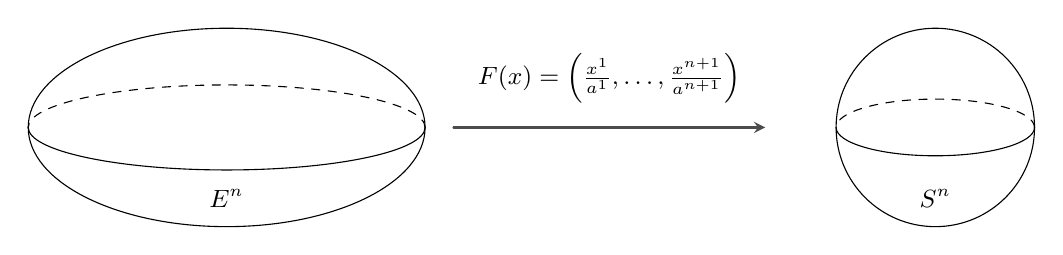
\begin{tikzpicture}[scale=1.8, line join=round, line cap=round]
			\tikzset{
				sphere_line/.style={thin, black},
				arrow/.style={->, >=stealth, thick, black!70},
				point/.style={circle, fill=black, inner sep=0.8pt}
			}
			% Elipsoide (S^n deformada)
			\draw[sphere_line] (0,0) ellipse (1.4 and 0.7);
			% Equador para efeito 3D
			\draw[dashed, sphere_line] (1.4, 0) arc (0:180:1.4 and 0.3);
			\draw[sphere_line] (1.4, 0) arc (0:-180:1.4 and 0.3); % Aqui corrigi para sphere_line
			\node[font=\small] at (0, -0.5) {$\mathbb{E}^n$};
			
			% Seta de transformação
			\draw[arrow] (1.6, 0) -- (3.8, 0);
			\node[above, font=\small] at (2.7, 0.1) {$F(x) = \left( \frac{x^1}{a^1}, \dots, \frac{x^{n+1}}{a^{n+1}} \right)$};
			
			% Esfera unitária
			\draw[sphere_line] (5,0) circle (0.7);
			% Equador para efeito 3D
			\draw[dashed, sphere_line] (5.7, 0) arc (0:180:0.7 and 0.2);
			\draw[sphere_line] (5.7, 0) arc (0:-180:0.7 and 0.2);
			\node[font=\small] at (5, -0.5) {$\mathbb{S}^n$};
		\end{tikzpicture}
		\caption{Difeomorfismo entre o elipsoide $\mathbb{E}^n$ e a esfera unitária $\mathbb{S}^n$ via a transformação linear de escala $F$.}
	\end{figure}
	
	\textbf{3. Prova de que $\mathbb{E}^n$ é uma Variedade Suave}
	
	Seja $f = F|_{\mathbb{E}^n} : \mathbb{E}^n \to \mathbb{S}^n$ a restrição de $F$ ao elipsoide. 
	\begin{enumerate}[label=(\roman*)]
		\item $f$ é suave, pois é a restrição de uma aplicação linear suave.
		\item $f$ é bijetiva, pois $F$ é um isomorfismo e $F(\mathbb{E}^n) = \mathbb{S}^n$.
		\item A inversa $f^{-1} = F^{-1}|_{\mathbb{S}^n}$ também é suave, pois é a restrição de uma aplicação linear suave.
	\end{enumerate}
	Assim, $f: \mathbb{E}^n \to \mathbb{S}^n$ é um \textbf{difeomorfismo}. 
	
	Como $\mathbb{S}^n$ é uma $n$-variedade suave (provado na Questão 3) e o difeomorfismo preserva a estrutura de variedade suave, concluímos que $\mathbb{E}^n$ também é uma $n$-variedade suave de dimensão $n$. A compacidade, a propriedade de Hausdorff e a base enumerável são herdadas de $\mathbb{S}^n$ via o difeomorfismo $f$.
}
%%%% QUESTÃO 06 %%%%
\questao{Mostre que superfícies regulares de $\mathbb{R}^3$ são 2-variedades suaves. Mais geralmente, mostre que hipersuperfícies regulares de $\mathbb{R}^{n+1}$ são $n$-variedades suaves.
}
\solucao{
	
	\textbf{Análise do Enunciado}
	\begin{itemize}
		\item \textbf{Hipóteses:} Uma hipersuperfície regular $M \subset \mathbb{R}^{n+1}$ definida por $f^{-1}(c)$ com $c$ sendo um valor regular de $f$.
		\item \textbf{Tese:} Provar que $M$ é uma $n$-variedade suave.
	\end{itemize}
	\vspace{5pt}
	\textbf{1. Definição de Hipersuperfície Regular}
	
	Uma hipersuperfície regular $M \subset \mathbb{R}^{n+1}$ é definida como o conjunto de pontos onde uma função suave $f: U \subseteq \mathbb{R}^{n+1} \to \mathbb{R}$ atinge um valor regular. Ou seja, existe um aberto $U \subseteq \mathbb{R}^{n+1}$ e um valor $c \in \mathbb{R}$ tal que:
	\[ M = f^{-1}(c) = \{ p \in U : f(p) = c \} \]
	A condição de ser \textbf{regular} implica que, para todo ponto $p \in M$, o diferencial $df_p : T_p\mathbb{R}^{n+1} \to T_{f(p)}\mathbb{R}$ é sobrejetivo. Como a dimensão do contradomínio é $1$, a sobrejetividade equivale a dizer que o gradiente de $f$ não se anula em $M$:
	\[ \nabla f(p) = \left( \frac{\partial f}{\partial x^1}(p), \dots, \frac{\partial f}{\partial x^{n+1}}(p) \right) \neq \vec{0}, \quad \forall p \in M. \]
	
	\textbf{2. Aplicação do Teorema do Valor Regular}
	
	De acordo com o Teorema do Valor Regular, se $f: U \to \mathbb{R}$ é uma aplicação suave e $c$ é um valor regular de $f$, então o conjunto nível $f^{-1}(c)$ é uma subvariedade suave de $U$ de codimensão $1$. 
	
	A dimensão de $M$ é dada por:
	\[ \dim(M) = \dim(\mathbb{R}^{n+1}) - \text{codim}(M) = (n+1) - 1 = n. \]
	Portanto, $M$ é uma $n$-variedade suave. Para o caso específico de superfícies em $\mathbb{R}^3$ ($n=2$), temos que $M$ é uma 2-variedade suave.
}
%%%% QUESTÃO 07 %%%%
\questao{Seja $\mathbb{B}^n = \left\{(x^1, \dots, x^n) \in \mathbb{R}^n : \sum_{i=1}^n (x^i)^2 < 1 \right\}$ a bola aberta unitária de $\mathbb{R}^n$. Prove que $\mathbb{B}^n$ é uma $n$-variedade suave. Além disso, mostre que $f : \mathbb{B}^n \to \mathbb{R}^n$ definida por $f(x) = \frac{x}{\sqrt{1-|x|^2}}$ é um difeomorfismo.
}
\solucao{
	
	\textbf{Análise do Enunciado}
	\begin{itemize}
		\item \textbf{Hipóteses:} $\mathbb{B}^n$ é a bola aberta unitária em $\mathbb{R}^n$.
		\item \textbf{Tese 1:} Provar que $\mathbb{B}^n$ é uma $n$-variedade suave.
		\item \textbf{Tese 2:} Provar que $f(x) = x/\sqrt{1-|x|^2}$ é um difeomorfismo entre $\mathbb{B}^n$ e $\mathbb{R}^n$.
	\end{itemize}
	\vspace{5pt}
	\textbf{1. Natureza de Variedade Suave de $\mathbb{B}^n$}
	
	Sendo $\mathbb{B}^n$ um subconjunto de $\mathbb{R}^n$, consideramos a topologia induzida. A função norma ao quadrado $g: \mathbb{R}^n \to \mathbb{R}$, dada por $g(x) = |x|^2 = \sum_{i=1}^n (x^i)^2$, é uma função contínua. Notemos que $\mathbb{B}^n = g^{-1}((-\infty, 1))$.
	
	Como $(-\infty, 1)$ é um aberto em $\mathbb{R}$, a imagem inversa $\mathbb{B}^n$ é um aberto de $\mathbb{R}^n$. 
	
	Sabemos que qualquer subconjunto aberto $U \subseteq \mathbb{R}^n$ é, por si só, uma $n$-variedade suave. O atlas suave para $\mathbb{B}^n$ é constituído por uma única carta $(\mathbb{B}^n, \text{Id})$, onde $\text{Id}: \mathbb{B}^n \to \mathbb{B}^n$ é a aplicação identidade. Como a identidade é infinitamente diferenciável, $\mathbb{B}^n$ é uma $n$-variedade suave.
	
	\textbf{2. Prova de que $f$ é um Difeomorfismo}
	
	Para que $f: \mathbb{B}^n \to \mathbb{R}^n$ seja um difeomorfismo, devemos provar que $f$ é bijetiva e que tanto $f$ quanto sua inversa $f^{-1}$ são suaves ($C^\infty$).
	
	\textbf{Suavidade de $f$:} A aplicação $f(x) = \frac{x}{\sqrt{1-|x|^2}}$ é composta por funções polinomiais e a função raiz quadrada. Como $|x|^2 < 1$ para todo $x \in \mathbb{B}^n$, o termo $1-|x|^2$ é estritamente positivo. A função $\sqrt{t}$ é suave para $t > 0$. Portanto, $f$ é a composição de funções suaves, sendo, portanto, suave em todo o seu domínio $\mathbb{B}^n$.
	
	\textbf{Cálculo da Inversa $f^{-1}$:} Seja $y \in \mathbb{R}^n$. Procuramos $x \in \mathbb{B}^n$ tal que $f(x) = y$. 
	Temos a relação:
	\[ y = \frac{x}{\sqrt{1-|x|^2}} \]
	Tomando a norma euclidiana de ambos os lados:
	\[ |y| = \frac{|x|}{\sqrt{1-|x|^2}} \implies |y|^2 = \frac{|x|^2}{1-|x|^2} \]
	Isolamos $|x|^2$:
	$$|y|^2(1-|x|^2)= |x|^2 \implies |y|^2 - |y|^2|x|^2 = |x|^2 \implies |y|^2 = |x|^2(1+|y|^2) \implies |x|^2 = \frac{|y|^2}{1+|y|^2}.$$
	Substituindo na equação original $x = y \sqrt{1-|x|^2}$, obtemos que:
	$$x = y \sqrt{1 - \frac{|y|^2}{1+|y|^2}} = y \sqrt{\frac{1+|y|^2 - |y|^2}{1+|y|^2}} = y \sqrt{\frac{1}{1+|y|^2}}=\frac{y}{\sqrt{1+|y|^2}}.$$
	Assim, a inversa $f^{-1}: \mathbb{R}^n \to \mathbb{B}^n$ é definida por $f^{-1}(y) = \frac{y}{\sqrt{1+|y|^2}}$.
	
	\textbf{Suavidade de $f^{-1}$:} Analogamente a $f$, a aplicação $f^{-1}$ é composta por funções suaves, pois o denominador $\sqrt{1+|y|^2}$ é sempre maior ou igual a $1$, nunca se anulando para qualquer $y \in \mathbb{R}^n$. Logo, $f^{-1}$ é suave.
	
	Como $f$ é uma bijecção suave com inversa suave, $f$ é um difeomorfismo entre a bola aberta $\mathbb{B}^n$ e o espaço euclidiano $\mathbb{R}^n$.
}
%%%% QUESTÃO 08 %%%%
\questao{Seja $GL(n, \mathbb{R}) = \{ A \in M(n, \mathbb{R}) : \det A \neq 0 \}$ o grupo linear geral das matrizes reais de ordem $n$. Mostre que $GL(n, \mathbb{R})$ é uma variedade suave. $GL(n, \mathbb{R})$ é conexo?
}
\solucao{
	
	\textbf{Análise do Enunciado}
	\begin{itemize}
		\item \textbf{Hipóteses:} $GL(n, \mathbb{R})$ é o conjunto das matrizes invertíveis.
		\item \textbf{Tese 1:} Provar que $GL(n, \mathbb{R})$ é uma variedade suave.
		\item \textbf{Tese 2:} Determinar se $GL(n, \mathbb{R})$ é um espaço conexo.
	\end{itemize}
	\vspace{5pt}
	\textbf{1. Prova de que $GL(n, \mathbb{R})$ é uma Variedade Suave}
	
	Consideremos o espaço de todas as matrizes reais de ordem $n$, denotado por $M(n, \mathbb{R})$. Este espaço é isomorfo ao espaço euclidiano $\mathbb{R}^{n^2}$ através da aplicação que mapeia cada matriz às suas componentes em um vetor coluna:
	\[ \Phi: M(n, \mathbb{R}) \to \mathbb{R}^{n^2}, \quad \Phi(A) = (A_{11}, A_{12}, \dots, A_{nn}) \]
	A função determinante $\det: M(n, \mathbb{R}) \to \mathbb{R}$ é um polinômio nas entradas da matriz $A_{ij}$. Como todo polinômio é uma função contínua, a aplicação $\det$ é contínua.
	
	Por definição, o grupo linear geral é o conjunto:
	\[ GL(n, \mathbb{R}) = \{ A \in M(n, \mathbb{R}) : \det A \neq 0 \} = \operatorname{det}^{-1}(\mathbb{R} \setminus \{0\}) \]
	O conjunto $\mathbb{R} \setminus \{0\}$ é um aberto no $\mathbb{R}$. Como a imagem inversa de um aberto por uma aplicação contínua é um aberto, concluímos que $GL(n, \mathbb{R})$ é um \textbf{subconjunto aberto} de $M(n, \mathbb{R}) \cong \mathbb{R}^{n^2}$.
	
	Concluímos que, o atlas suave para $GL(n, \mathbb{R})$ é constituído por uma única carta $(GL(n, \mathbb{R}), \text{Id})$. Portanto, $GL(n, \mathbb{R})$ é uma $n^2$-variedade suave.
	
	\textbf{2. Análise da Conexidade}
	
	Para analisar se $GL(n, \mathbb{R})$ é conexo, consideramos novamente a aplicação determinante $\det: GL(n, \mathbb{R}) \to \mathbb{R} \setminus \{0\}$. Sabemos que:
	\begin{enumerate}[label=(\roman*)]
		\item A aplicação $\det$ é contínua.
		\item O contradomínio $\mathbb{R} \setminus \{0\}$ é a união de dois abertos disjuntos: $(-\infty, 0) \cup (0, \infty)$.
	\end{enumerate}
	Se $GL(n, \mathbb{R})$ fosse conexo, a sua imagem sob uma aplicação contínua também deveria ser conexa. No entanto, a imagem da aplicação $\det$ é todo o conjunto $\mathbb{R} \setminus \{0\}$, que é desconexo. 
	
	Podemos definir dois subconjuntos:
	\[ GL^+(n, \mathbb{R}) = \{ A \in GL(n, \mathbb{R}) : \det A > 0 \} \quad \text{e} \quad GL^-(n, \mathbb{R}) = \{ A \in GL(n, \mathbb{R}) : \det A < 0 \} \]
	Ambos são abertos em $GL(n, \mathbb{R})$ (pois são imagens inversas de abertos do $\mathbb{R}$) e são disjuntos. 
	
	Como $GL(n, \mathbb{R}) = GL^+(n, \mathbb{R}) \cup GL^-(n, \mathbb{R})$, temos que $GL(n, \mathbb{R})$ é a união de dois abertos disjuntos não vazios. Portanto, $GL(n, \mathbb{R})$ é \textbf{desconexo}.
}
%%%% QUESTÃO 09 %%%%
\questao{Seja $O(n) = \{A \in M(n, \mathbb{R}) : AA^t = I\}$ o grupo das matrizes ortogonais reais de ordem $n$. Mostre que $O(n)$ é uma variedade suave, compacta e de Hausdorff com base enumerável de dimensão $\frac{n(n-1)}{2}$.
}
\solucao{
	
	\textbf{Análise do Enunciado}
	\begin{itemize}
		\item \textbf{Hipóteses:} $O(n)$ é o conjunto de matrizes tais que $AA^t = I$.
		\item \textbf{Tese:} Provar que $O(n)$ é uma variedade suave, compacta, Hausdorff, com base enumerável e dimensão $n(n-1)/2$.
	\end{itemize}
	\vspace{5pt}
	\textbf{1. Construção via Teorema do Valor Regular}
	
	Consideremos o espaço de todas as matrizes reais $M(n, \mathbb{R})$, que é isomorfo ao espaço euclidiano $\mathbb{R}^{n^2}$. Definimos o espaço das matrizes simétricas $S(n, \mathbb{R}) = \{ S \in M(n, \mathbb{R}) : S = S^t \}$. 
	
	\textbf{Cálculo da Dimensão de $S(n, \mathbb{R})$:} Uma matriz simétrica é completamente determinada por suas entradas na diagonal principal e por suas entradas acima da diagonal.
	\begin{itemize}
		\item Existem $n$ entradas na diagonal principal: $S_{11}, S_{22}, \dots, S_{nn}$.
		\item Existem $\frac{n(n-1)}{2}$ entradas acima da diagonal principal.
	\end{itemize}
	Assim, a dimensão de $S(n, \mathbb{R})$ é a soma desses valores:
	\[ \dim(S(n, \mathbb{R})) = n + \frac{n(n-1)}{2} = \frac{2n + n^2 - n}{2} = \frac{n(n+1)}{2}. \]
	
	Definimos a aplicação suave $F: M(n, \mathbb{R}) \to S(n, \mathbb{R})$ dada por:
	\[ F(A) = AA^t \]
	Note que $F(A)$ é sempre simétrica, pois $(AA^t)^t = (A^t)^t A^t = AA^t$. O grupo ortogonal é, por definição, a imagem inversa do valor $I \in S(n, \mathbb{R})$:
	\[ O(n) = F^{-1}(I). \]
	
	\textbf{Prova de que $I$ é um Valor Regular:} Para cada $A \in O(n)$, devemos mostrar que o diferencial $$dF_A: T_A M(n, \mathbb{R}) \to T_{F(A)} S(n, \mathbb{R}),$$ é sobrejetivo. Identificando os espaços tangentes com as próprias matrizes, seja $H \in M(n, \mathbb{R})$. O diferencial é calculado via a derivada direcional:
	\begin{align*}
		dF_A(H) &= \lim_{t \to 0} \frac{F(A+tH) - F(A)}{t} \\
		&= \lim_{t \to 0} \frac{(A+tH)(A+tH)^t - AA^t}{t} \\
		&= \lim_{t \to 0} \frac{AA^t + t(AH^t + HA^t) + t^2 HH^t - AA^t}{t} \\
		&= AH^t + HA^t.
	\end{align*}
	Para provar a sobrejetividade, dado qualquer $S \in S(n, \mathbb{R})$, devemos encontrar $H$ tal que $AH^t + HA^t = S$. Escolhemos $H = \frac{1}{2}SA$. Então $H^t = \frac{1}{2}A^t S^t = \frac{1}{2}A^t S$ (pois $S$ é simétrica). Substituindo:
	$$ dF_A(H) = A\left(\frac{1}{2}A^t S\right) + \left(\frac{1}{2}SA\right)A^t = \frac{1}{2}AA^t S + \frac{1}{2}S AA^t=\frac{1}{2}IS + \frac{1}{2}SI = S,$$
	pois $A \in O(n)$.
	
	Como $dF_A$ é sobrejetivo para todo $A \in O(n)$, o valor $I$ é um valor regular. Pelo Teorema do Valor Regular, $O(n)$ é uma subvariedade suave de $M(n, \mathbb{R})$.
	
	\textbf{Cálculo da Dimensão: }A dimensão de $O(n, \mathbb{R})$ é a dimensão do espaço ambiente menos a dimensão do contradomínio da função $F$, ou seja, 
	$$\dim(O(n)) = \dim(M(n, \mathbb{R})) - \dim(S(n, \mathbb{R})) = n^2 - \frac{n(n+1)}{2} = \frac{2n^2 - n^2 - n}{2} = \frac{n(n-1)}{2}.$$
	
	\textbf{2. Propriedades Topológicas}
	
	\textbf{Hausdorff e Base Enumerável:} Como $O(n) \subset M(n, \mathbb{R}) \cong \mathbb{R}^{n^2}$, essas propriedades são herdadas diretamente da topologia induzida do espaço euclidiano.
	
	\textbf{Compacidade:} $O(n)$ é um subconjunto fechado de $M(n, \mathbb{R})$ por ser a imagem inversa do ponto $\{I\}$ sob a aplicação contínua $F$. Para provar que é limitado, observemos que para qualquer $A \in O(n)$, as linhas de $A$ são vetores ortonormais em $\mathbb{R}^n$. Se denotarmos por $r_i$ a $i$-ésima linha de $A$, temos $|r_i|^2 = \sum_{j=1}^n A_{ij}^2 = 1$ para todo $i \in \{1, \dots, n\}$. A soma de todos os quadrados das componentes de $A$ é, portanto:
	\[ \sum_{i=1}^n \sum_{j=1}^n A_{ij}^2 = \sum_{i=1}^n |r_i|^2 = \sum_{i=1}^n 1 = n. \]
	Isso implica que todo $A \in O(n)$ satisfaz $|A|^2 = n$, ou seja, $O(n)$ está contido na esfera de raio $\sqrt{n}$ em $\mathbb{R}^{n^2}$. Como qualquer esfera em $\mathbb{R}^{n^2}$ é um conjunto limitado, $O(n)$ é limitado. Pelo Teorema de Heine-Borel, $O(n)$ é compacto.
}
%%%% QUESTÃO 10 %%%%
\questao{Seja $SL(n, \mathbb{R}) = \{ A \in M(n, \mathbb{R}) : \det A = 1 \}$. Mostre que $SL(n, \mathbb{R})$ é uma variedade suave.
}
\solucao{
	
	\textbf{Análise do Enunciado}
	\begin{itemize}
		\item \textbf{Hipóteses:} $SL(n, \mathbb{R})$ é o conjunto de matrizes com determinante igual a 1.
		\item \textbf{Tese:} Provar que $SL(n, \mathbb{R})$ é uma variedade suave.
	\end{itemize}
	\vspace{5pt}
	\textbf{1. Construção via Teorema do Valor Regular}
	
	Consideremos o espaço de todas as matrizes reais de ordem $n$, $M(n, \mathbb{R})$, que é isomorfo ao espaço euclidiano $\mathbb{R}^{n^2}$. Definimos a aplicação determinante:
	\[ f: M(n, \mathbb{R}) \to \mathbb{R}, \quad f(A) = \det(A) \]
	A função determinante é um polinômio nas entradas da matriz $A_{ij}$, sendo, portanto, uma aplicação suave ($C^\infty$). O Grupo Linear Especial $SL(n, \mathbb{R})$ é, por definição, a imagem inversa do valor $1 \in \mathbb{R}$:
	\[ SL(n, \mathbb{R}) = f^{-1}(1) \]
	
	\textbf{2. Análise do Valor Regular e o Diferencial do Determinante}
	
	Para provar que $SL(n, \mathbb{R})$ é uma variedade suave, devemos mostrar que $1$ é um valor regular de $f$. Isso exige que, para todo $A \in SL(n, \mathbb{R})$, o diferencial $df_A: T_A M(n, \mathbb{R}) \to T_{f(A)} \mathbb{R}$ seja sobrejetivo. 
	
	Identificando $T_A M(n, \mathbb{R}) \cong M(n, \mathbb{R})$, tomemos uma matriz $H \in M(n, \mathbb{R})$. O diferencial do determinante no ponto $A$ é dado pela \textbf{Fórmula de Jacobi}:
	\[ df_A(H) = \text{tr}(\text{adj}(A) H) \]
	onde $\text{adj}(A)$ é a matriz adjunta de $A$. Como $A \in SL(n, \mathbb{R})$, sabemos que $A$ é invertível ($\det A = 1$) e que $\text{adj}(A) = \det(A) A^{-1} = A^{-1}$. Assim, o diferencial simplifica-se para:
	\[ df_A(H) = \text{tr}(A^{-1} H) \]
	
	\textbf{Prova de Sobrejetividade:} Para que $df_A$ seja sobrejetivo, dado qualquer $\lambda \in \mathbb{R}$, devemos encontrar uma matriz $H$ tal que $\text{tr}(A^{-1}H) = \lambda$. Escolhemos a matriz $H = \frac{\lambda}{n} A$. Então:
	\[ df_A(H) = \text{tr}(A^{-1} \cdot \frac{\lambda}{n} A) = \text{tr}(\frac{\lambda}{n} I) = \frac{\lambda}{n} \text{tr}(I) = \frac{\lambda}{n} \cdot n = \lambda \]
	Como $df_A$ é sobrejetivo para todo $A \in SL(n, \mathbb{R})$, $1$ é um valor regular de $f$. Pelo Teorema do Valor Regular, $SL(n, \mathbb{R})$ é uma subvariedade suave de $M(n, \mathbb{R})$.
	
	\textbf{Cálculo da Dimensão:}
	A dimensão de $SL(n, \mathbb{R})$ é a dimensão do espaço ambiente menos a dimensão do contradomínio da função $f$, ou seja, $\dim(SL(n, \mathbb{R})) = \dim(M(n, \mathbb{R})) - \dim(\mathbb{R}) = n^2 - 1$.
}
%%%% QUESTÃO 11 %%%%
\questao{ \textbf{(Construção de variedades suaves)} Seja $M$ um subconjunto. Suponha que são dados uma coleção $\{U_\alpha\}_{\alpha \in \Lambda}$ de subconjuntos de $M$ junto com uma aplicação injetiva $\varphi_\alpha : U_\alpha \to \mathbb{R}^n$, para cada $\alpha \in \Lambda$, tais que as seguintes propriedades são satisfeitas:
	\begin{enumerate}[label=(\alph*)]
		\item Para cada $\alpha \in \Lambda$, $\varphi_\alpha(U_\alpha)$ é um subconjunto aberto de $\mathbb{R}^n$.
		\item Para cada par $\alpha, \beta \in \Lambda$, $\varphi_\alpha(U_\alpha \cap U_\beta)$ e $\varphi_\beta(U_\alpha \cap U_\beta)$ são abertos em $\mathbb{R}^n$.
		\item Quando $U_\alpha \cap U_\beta \neq \emptyset$, $\varphi_\alpha \circ \varphi_\beta^{-1} : \varphi_\beta(U_\alpha \cap U_\beta) \to \varphi_\alpha(U_\alpha \cap U_\beta)$ é um difeomorfismo.
		\item Quantidades contáveis de subconjuntos $U_\alpha$ cobrem $M$.
		\item Quando $p,q$ são pontos distintos de $M$, ou existe algum $U_\alpha$ contendo $p$ e $q$ ou existem conjuntos disjuntos $U_\alpha$ e $U_\beta$ tais que $p \in U_\alpha$ e $q \in U_\beta$.
	\end{enumerate}
	Mostre que $M$ admite uma única estrutura suave de forma que $(U_\alpha, \varphi_\alpha)$ seja uma carta suave.
}
\solucao{
	
	\textbf{Análise do Enunciado}
	\begin{itemize}
		\item \textbf{Hipóteses:} Um conjunto $M$ com uma coleção de aplicações injetivas $\varphi_\alpha$ satisfazendo cinco condições (abertos em $\mathbb{R}^n$, transições difeomórficas, cobertura contável e separabilidade de pontos).
		\item \textbf{Tese:} Provar que $M$ possui uma única estrutura de variedade suave induzida por essas cartas.
	\end{itemize}
	\vspace{5pt}
	\textbf{1. Definição da Topologia em $M$}
	
	Para que $M$ seja uma variedade, devemos primeiro definir uma topologia sobre ele. Definimos que um subconjunto $V \subseteq M$ é \textbf{aberto} se, e somente se, para todo $\alpha \in \Lambda$, a imagem $\varphi_\alpha(V \cap U_\alpha)$ for um aberto em $\mathbb{R}^n$.
	
	Verifiquemos que isso define uma topologia:
	\begin{enumerate}[label=(\roman*)]
		\item $\emptyset$ e $M$ são abertos, pois $\varphi_\alpha(\emptyset) = \emptyset$ e $\varphi_\alpha(M \cap U_\alpha) = \varphi_\alpha(U_\alpha)$, que são abertos em $\mathbb{R}^n$ por hipótese (a).
		\item A união arbitrária de abertos $\bigcup V_i$ é aberta, pois $\varphi_\alpha\left(\left(\bigcup V_i\right) \cap U_\alpha\right) = \bigcup (\varphi_\alpha\left(V_i \cap U_\alpha\right))$, que é união de abertos.
		\item A interseção finita de abertos $V_1 \cap V_2$ é aberta, pois $\varphi_\alpha((V_1 \cap V_2) \cap U_\alpha) = \varphi_\alpha(V_1 \cap U_\alpha) \cap \varphi_\alpha(V_2 \cap U_\alpha)$, que é a interseção de dois abertos em $\mathbb{R}^n$.
	\end{enumerate}
	Assim, $M$ é um espaço topológico e cada $\varphi_\alpha : U_\alpha \to \varphi_\alpha(U_\alpha)$ é, por construção, um homeomorfismo.
	
	\textbf{2. Propriedade de Hausdorff}
	
	Sejam $p, q \in M$ pontos distintos. Devemos encontrar abertos disjuntos $V_p$ e $V_q$ contendo $p$ e $q$, respectivamente. Pela hipótese (e), temos dois casos:
	\begin{itemize}
		\item \textbf{Caso 1:} $p, q$ pertencem ao mesmo $U_\alpha$. Como $\varphi_\alpha(U_\alpha)$ é um aberto de $\mathbb{R}^n$ (Hausdorff), existem abertos disjuntos $W_p, W_q \subset \varphi_\alpha(U_\alpha)$ tais que $\varphi_\alpha(p) \in W_p$ e $\varphi_\alpha(q) \in W_q$. Então, $V_p = \varphi_\alpha^{-1}(W_p)$ e $V_q = \varphi_\alpha^{-1}(W_q)$ são abertos disjuntos em $M$ contendo $p$ e $q$.
		\item \textbf{Caso 2:} Existem $U_\alpha, U_\beta$ disjuntos tais que $p \in U_\alpha$ e $q \in U_\beta$. Como $U_\alpha \cap U_\beta = \emptyset$, estes já são os abertos disjuntos necessários.
	\end{itemize}
	Portanto, $M$ é um espaço de Hausdorff.
	
	\textbf{3. Base Enumerável}
	
	Pela hipótese (d), a coleção $\{U_\alpha\}_{\alpha \in \Lambda}$ é contável. Para cada $\alpha$, a imagem $\varphi_\alpha(U_\alpha)$ é um aberto de $\mathbb{R}^n$, que possui uma base enumerável de bolas abertas $\{B_{\alpha, n}\}_{n \in \mathbb{N}}$. A coleção $\{\varphi_\alpha^{-1}(B_{\alpha, n}) : \alpha \in \Lambda, n \in \mathbb{N}\}$ é uma união contável de coleções enumeráveis, logo é uma base enumerável para a topologia de $M$.
	
	\textbf{4. Estrutura Suave e Unicidade}
	
	Temos agora que $M$ é um espaço de Hausdorff com base enumerável e que a coleção $\mathcal{A} = \{(U_\alpha, \varphi_\alpha)\}_{\alpha \in \Lambda}$ cobre $M$. A hipótese (c) garante que para quaisquer $\alpha, \beta \in \Lambda$, a função de transição $\varphi_\alpha \circ \varphi_\beta^{-1}$ é um difeomorfismo entre abertos de $\mathbb{R}^n$. Portanto, por definição, $\mathcal{A}$ é um atlas suave para $M$.
	
	Para a unicidade da estrutura suave, recorremos ao resultado provado na \textbf{Questão 1}. Vimos que qualquer atlas suave está contido em um único atlas suave maximal. Sendo $\mathcal{A}$ um atlas suave, existe um único atlas maximal $\mathcal{A}_{max}$ tal que $\mathcal{A} \subseteq \mathcal{A}_{max}$. 
	
	Uma estrutura suave em uma variedade é definida precisamente como a classe de equivalência de atlas suaves que compartilham o mesmo atlas maximal. Como a coleção $\{(U_\alpha, \varphi_\alpha)\}_{\alpha \in \Lambda}$ determina um único $\mathcal{A}_{max}$, a estrutura suave induzida em $M$ é única. Concluímos, portanto, que $M$ é uma $n$-variedade suave.
}
%%%% QUESTÃO 12 %%%%
\questao{ \textbf{(Orientabilidade)} Seja $(M^n, \mathcal{A})$ uma $n$-variedade suave. Dizemos que $M^n$ é orientável se $M^n$ pode ser coberta por um atlas $\{U_\alpha, \varphi_\alpha\}_{\alpha \in \Lambda} \subset \mathcal{A}$ tal que para todo par $\alpha, \beta \in \Lambda$ com $U_\alpha \cap U_\beta \neq \emptyset$, a derivada da aplicação transição $\varphi_\beta \circ \varphi_\alpha^{-1}$ tem determinante positivo. Caso tal atlas não exista, dizemos que $M^n$ é não-orientável.
	\begin{enumerate}[label=(\alph*)]
		\item Mostre que se uma $n$-variedade suave $M^n$ pode ser coberta por duas vizinhanças coordenadas $U_1$ e $U_2$ de modo que a interseção $U_1 \cap U_2$ é conexa, então $M^n$ é orientável.
		\item Use item (a) para mostrar que $\mathbb{S}^n$ é orientável.
		\item Mostre diretamente que $\mathbb{RP}^2$ é não-orientável.
\end{enumerate}
}
\solucao{
	
	\textbf{Análise do Enunciado}
	\begin{itemize}
		\item \textbf{Hipóteses:} Definição de orientabilidade via sinal do determinante da Jacobiana das transições.
		\item \textbf{Tese (a):} Provar que a conexidade da interseção de dois abertos de cobertura implica orientabilidade.
		\item \textbf{Tese (b):} Aplicar o resultado (a) à esfera $\mathbb{S}^n$.
		\item \textbf{Tese (c):} Demonstrar a não-orientabilidade de $\mathbb{RP}^2$.
	\end{itemize}
	\vspace{5pt}
	\textbf{(a) Prova da Orientabilidade via Interseção Conexa}
	
	Sejam $(U_1, \varphi_1)$ e $(U_2, \varphi_2)$ as duas cartas que cobrem $M^n$. A aplicação de transição é $\tau = \varphi_2 \circ \varphi_1^{-1}$, definida no aberto $W = \varphi_1(U_1 \cap U_2) \subset \mathbb{R}^n$. 
	
	Consideremos a função determinante do Jacobiano $J_\tau: W \to \mathbb{R}$, dada por $J_\tau(u) = \det(d\tau_u)$. Como $\tau$ é um difeomorfismo, $d\tau_u$ é invertível para todo $u \in W$, logo $J_\tau(u) \neq 0$ para todo $u \in W$.
	
	Por hipótese, $U_1 \cap U_2$ é conexo. Como $\varphi_1$ é um homeomorfismo, a imagem $W = \varphi_1(U_1 \cap U_2)$ também é um conjunto conexo em $\mathbb{R}^n$. A função $J_\tau$ é contínua e nunca se anula em $W$. Pelo Teorema do Valor Intermediário, uma função contínua em um conjunto conexo que nunca assume o valor zero deve manter o mesmo sinal em todo o domínio.
	
	Existem dois casos:
	\begin{enumerate}[label=(\roman*)]
		\item Se $J_\tau(u) > 0$ para todo $u \in W$, o atlas $\{(U_1, \varphi_1), (U_2, \varphi_2)\}$ já é um atlas de orientação.
		\item Se $J_\tau(u) < 0$ para todo $u \in W$, definimos uma nova carta $(U_1, \tilde{\varphi}_1)$ onde $\tilde{\varphi}_1(x) = (-\varphi_1^1(x), \varphi_1^2(x), \dots, \varphi_1^n(x))$. A nova transição será $\tau' = \varphi_2 \circ \tilde{\varphi}_1^{-1}$. A matriz Jacobiana de $\tilde{\varphi}_1$ é $\text{diag}(-1, 1, \dots, 1)$, com determinante $-1$. Pela regra da cadeia:
		\[ \det(d\tau'_u) = \det(d(\varphi_2 \circ \varphi_1^{-1})_u) \cdot \det(d\tilde{\varphi}_1^{-1}) = J_\tau(u) \cdot (-1) > 0. \]
	\end{enumerate}
	Em ambos os casos, construímos um atlas onde a transição tem determinante positivo. Logo, $M^n$ é orientável.
	
	\textbf{(b) Orientabilidade da Esfera $\mathbb{S}^n$}
	
	Utilizaremos a construção da \textbf{Questão 3(c)}, onde $\mathbb{S}^n$ é coberta pelas duas cartas de projeção estereográfica $(U_N, \phi_N)$ e $(U_S, \phi_S)$. 
	
	A interseção dos domínios é dada por $U_N \cap U_S = \mathbb{S}^n \setminus \{N, S\}$. Para analisar a conexidade deste conjunto, observamos que a projeção $\phi_N$ restrita a essa interseção é um homeomorfismo:
	\[ \phi_N : \mathbb{S}^n \setminus \{N, S\} \longrightarrow \mathbb{R}^n \setminus \{0\} \]
	Sendo $\mathbb{R}^n \setminus \{0\}$ homeomorfo ao produto $\mathbb{S}^{n-1} \times (0, \infty)$ via a aplicação $v \mapsto \left( \frac{v}{|v|}, |v| \right)$, e considerando que $(0, \infty) \cong \mathbb{R}$, concluímos que:
	\[ U_N \cap U_S \cong \mathbb{S}^{n-1} \times \mathbb{R} \]
	Para $n \ge 2$, a esfera $\mathbb{S}^{n-1}$ é conexa e, como o produto de espaços conexos é conexo, a interseção $U_N \cap U_S$ é conexa. Sendo a interseção conexa, a condição do item (a) é satisfeita. Portanto, $\mathbb{S}^n$ é orientável.
	
	\textbf{(c) Não-orientabilidade de $\mathbb{RP}^2$}
	
	Utilizaremos as cartas $\phi_i$ definidas na \textbf{Questão 4}. Consideremos as cartas $\phi_1$ e $\phi_2$ nos abertos $U_1$ e $U_2$. Para $n=2$, as coordenadas são $\phi_1([x]) = (x^2/x^1, x^3/x^1)$ e $\phi_2([x]) = (x^1/x^2, x^3/x^2)$.
	
	A transição $\tau = \phi_2 \circ \phi_1^{-1}$ no domínio $u = (u^1, u^2) \in \mathbb{R}^2 \setminus \{0\}$ é:
	\[ \tau(u^1, u^2) = \left( \frac{1}{u^1}, \frac{u^2}{u^1} \right) \]
	Calculamos a matriz Jacobiana $d\tau$:
	\[ d\tau = \begin{bmatrix} 
		\frac{\partial \tau^1}{\partial u^1} & \frac{\partial \tau^1}{\partial u^2} \\ 
		\\
		\frac{\partial \tau^2}{\partial u^1} & \frac{\partial \tau^2}{\partial u^2} \end{bmatrix} = \begin{bmatrix} 
		\frac{-1}{(u^1)^2} & 0 \\
		\\
		\frac{-u^2}{(u^1)^2} & \frac{1}{u^1} \end{bmatrix} \]
	O determinante da transição é:
	\[ \det(d\tau) = \left( -\frac{1}{(u^1)^2} \right) \left( \frac{1}{u^1} \right) - 0 = -\frac{1}{(u^1)^3} \]
	Observe que o sinal do determinante depende do sinal de $u^1$. No domínio $\phi_1(U_1 \cap U_2) = \mathbb{R}^2 \setminus \{0\}$, a coordenada $u^1$ pode assumir tanto valores positivos quanto negativos. 
	
	Se tentarmos mudar a orientação de $\phi_1$ ou $\phi_2$ multiplicando uma coordenada por $-1$, alteraremos o sinal do determinante em todo o domínio. No entanto, como o sinal de $\det(d\tau)$ varia dentro do mesmo domínio de transição (ele é positivo para $u^1 < 0$ e negativo para $u^1 > 0$), não existe escolha de sinais para as cartas que torne o determinante globalmente positivo. Portanto, $\mathbb{RP}^2$ é não-orientável.
}
%%%% QUESTÃO 13 %%%%
\questao{Sejam $M^n$ uma variedade suave e $f : M^n \to \mathbb{R}^k$ uma aplicação suave. Mostre que a representação coordenada $\hat{f}$ de $f$ é suave para qualquer carta suave $(U, \varphi)$ de $M^n$.
}
\solucao{
	
	\textbf{Análise do Enunciado}
	\begin{itemize}
		\item \textbf{Hipóteses:} $f$ é uma aplicação suave de uma variedade $M^n$ para $\mathbb{R}^k$.
		\item \textbf{Tese:} Provar que a representação local $\hat{f} = f \circ \varphi^{-1}$ é suave.
	\end{itemize}
	\vspace{5pt}
	\textbf{1. Definições e Notação}
	
	Seja $(U, \varphi)$ uma carta suave de $M^n$. A representação coordenada de $f$ em relação a esta carta é a aplicação $\hat{f} : \varphi(U) \to \mathbb{R}^k$ definida pela composição:
	\[ \hat{f} = f \circ \varphi^{-1} \]
	onde $\varphi(U)$ é um aberto em $\mathbb{R}^n$ e a aplicação $\varphi^{-1}: \varphi(U) \to U$ é o homeomorfismo inverso da carta.
	
	\textbf{2. Análise da Suavidade}
	
	Para provar que $\hat{f}$ é suave, analisamos a sequência de aplicações:
	\[ \mathbb{R}^n \xrightarrow{\varphi^{-1}} M^n \xrightarrow{f} \mathbb{R}^k \]
	Pela definição de estrutura suave em $M^n$, a aplicação $\varphi^{-1}$ é suave. Como, por hipótese, $f$ é uma aplicação suave de $M^n$ para $\mathbb{R}^k$, a composição $\hat{f} = f \circ \varphi^{-1}$ é a composição de duas aplicações suaves entre variedades. 
	
	Sendo a composição de funções suaves também suave, concluímos que $\hat{f} \in C^\infty(\varphi(U), \mathbb{R}^k)$.
	
	\textbf{3. Independência da Escolha da Carta}
	
	Para garantir a consistência da definição, consideremos outra carta $(V, \psi)$ tal que $U \cap V \neq \emptyset$. A representação de $f$ em relação a $\psi$, denotada por $\tilde{f} = f \circ \psi^{-1}$, relaciona-se com $\hat{f}$ através da função de transição $\tau_{\psi\varphi} = \varphi \circ \psi^{-1}$:
	\[ \tilde{f} = f \circ \psi^{-1} = \underbrace{(f \circ \varphi^{-1})}_{\hat{f}} \circ \underbrace{(\varphi \circ \psi^{-1})}_{\tau_{\psi\varphi}} = \hat{f} \circ \tau_{\psi\varphi} \]
	Como $\tau_{\psi\varphi}$ é um difeomorfismo entre abertos de $\mathbb{R}^n$ e $\hat{f}$ é suave, a composição $\tilde{f}$ é necessariamente suave. Isso prova que a suavidade da representação coordenada é uma propriedade intrínseca da aplicação $f$, independente da carta escolhida.
}
%%%% QUESTÃO 14 %%%%
\questao{
	Sejam $M^{n}$ e $N^{k}$ variedades suaves, e seja $\{U_{\alpha}\}_{\alpha \in \Gamma}$ uma cobertura de $M^{n}$. Suponha que para cada $\alpha \in \Gamma$ temos uma aplicação suave $F_{\alpha} : U_{\alpha} \to N^{k}$ tal que $F_{\alpha} \big|_{U_{\alpha} \cap U_{\beta}} = F_{\beta} \big|_{U_{\alpha} \cap U_{\beta}}$, para quaisquer $\alpha, \beta \in \Gamma$. Mostre que existe uma única aplicação $F : M^{n} \to N^{k}$ tal que $F \big|_{U_{\alpha}} = F_{\alpha}$, para todo $\alpha \in \Gamma$.
}
\solucao{
	
	\textbf{Análise do Enunciado}
	\begin{itemize}
		\item \textbf{Hipóteses:} $\{U_\alpha\}$ cobre $M^n$, e cada $F_\alpha: U_\alpha \to N^k$ é suave e compatível nas interseções.
		\item \textbf{Tese:} Existência e unicidade de uma aplicação global $F: M^n \to N^k$ que seja suave.
	\end{itemize}
	\vspace{5pt}
	\textbf{1. Existência e Boa Definição de $F$:}
	Definimos a aplicação $F: M^n \to N^k$ da seguinte forma: para qualquer ponto $p \in M^n$, como $\{U_\alpha\}_{\alpha \in \Gamma}$ é uma cobertura de $M^n$, existe pelo menos um índice $\alpha \in \Gamma$ tal que $p \in U_\alpha$. Atribuímos:
	\begin{equation*}
		F(p) = F_\alpha(p).
	\end{equation*}
	Para que $F$ esteja bem definida, o valor de $F(p)$ não deve depender da escolha do índice $\alpha$. Seja $p \in U_\alpha \cap U_\beta$. Pela hipótese de compatibilidade, temos que:
	\begin{equation*}
		F_\alpha \big|_{U_\alpha \cap U_\beta} = F_\beta \big|_{U_\alpha \cap U_\beta} \implies F_\alpha(p) = F_\beta(p).
	\end{equation*}
	Portanto, a aplicação $F$ é bem definida em todo o domínio $M^n$.
	
	\textbf{2. Unicidade:}
	Suponha que exista outra aplicação $G: M^n \to N^k$ tal que $G \big|_{U_\alpha} = F_\alpha$ para todo $\alpha \in \Gamma$. Para qualquer $p \in M^n$, escolhemos $\alpha$ tal que $p \in U_\alpha$. Então:
	$$G(p) = G \big|_{U_\alpha}(p) = F_\alpha(p) = F(p).$$
	Como $G(p) = F(p)$ para todo $p \in M^n$, concluímos que $G = F$.
	
	\textbf{3. Suavidade de $F$:}
	Para provar que $F$ é suave, devemos verificar a condição de suavidade em cada ponto $p \in M^n$. 
	Seja $p \in M^n$. Existe um índice $\alpha \in \Gamma$ tal que $p \in U_\alpha$. Por hipótese, a aplicação $F_\alpha: U_\alpha \to N^k$ é suave. 
	
	Pela definição de suavidade em $U_\alpha$, para o ponto $p$, existem cartas coordenadas $(U_p, \varphi)$ em $M^n$ com $p \in U_p \subseteq U_\alpha$ e $(V_{F(p)}, \psi)$ em $N^k$ com $F(p) \in V_{F(p)}$ tais que a representação coordenada de $F_\alpha$ no ponto $p$:
	\begin{equation*}
		\hat{F}_\alpha = \psi \circ F_\alpha \circ \varphi^{-1}
	\end{equation*}
	é uma aplicação suave de $\varphi(U_p) \subseteq \mathbb{R}^n$ em $\psi(V_{F(p)}) \subseteq \mathbb{R}^k$.
	
	Como $F \big|_{U_\alpha} = F_\alpha$, temos que:
	\begin{equation*}
		\psi \circ F \circ \varphi^{-1} = \psi \circ (F \big|_{U_\alpha}) \circ \varphi^{-1} = \psi \circ F_\alpha \circ \varphi^{-1} = \hat{F}_\alpha.
	\end{equation*}
	Assim, $\hat{F}_\alpha$ é suave para todo $p \in M^n$, e portanto a aplicação global $F$ satisfaz a definição de aplicação suave entre variedades.
	
	A aplicação $F$ foi construída a partir de dados locais compatíveis, é única por construção e sua suavidade decorre da suavidade local de cada $F_\alpha$. Assim, $F$ é a única aplicação suave que estende a coleção $\{F_\alpha\}$.
}
%%%% QUESTÃO 15 %%%%
\questao{
	Sejam $M^{n}$ e $N^{k}$ variedades suaves e $F : M^{n} \to N^{k}$ uma aplicação suave. Mostre que a representação coordenada $\hat{F}$ de $F$ é suave para qualquer par de cartas coordenadas suaves $(U, \varphi)$ de $M^{n}$ e $(V, \psi)$ de $N^{k}$, respectivamente.
}
\solucao{
	
	\textbf{Análise do Enunciado}
	\begin{itemize}
		\item \textbf{Hipóteses:} $F$ é uma aplicação suave entre as variedades $M^n$ e $N^k$.
		\item \textbf{Tese:} Provar que a representação coordenada $\hat{F} = \psi \circ F \circ \varphi^{-1}$ é suave para qualquer escolha de cartas.
	\end{itemize}
	\vspace{5pt}
	Seja $\hat{F} = \psi \circ F \circ \varphi^{-1}$ a representação coordenada de $F$ em relação às cartas $(U, \varphi)$ e $(V, \psi)$. O domínio de $\hat{F}$ é o aberto $\varphi(U \cap F^{-1}(V)) \subseteq \mathbb{R}^n$. 
	
	\textbf{1. Existência de representação local suave:}
	Seja $p \in U \cap F^{-1}(V)$. Como $F$ é uma aplicação suave, por definição, existe um par de cartas $(U', \varphi')$ em $M^n$ e $(V', \psi')$ em $N^k$ tais que $p \in U'$, $F(p) \in V'$ e a representação coordenada local
	\begin{equation*}
		\tilde{F} = \psi' \circ F \circ (\varphi')^{-1}
	\end{equation*}
	é suave em uma vizinhança de $\varphi'(p)$.
	
	\textbf{2. Decomposição via funções de transição:}
	Para formalizar o domínio de validade desta composição, definimos o aberto $W = U \cap U' \cap F^{-1}(V \cap V')$. Como $U$ e $U'$ são abertos em $M^n$, $V$ e $V'$ são abertos em $N^k$ e $F$ é contínua, $W$ é uma vizinhança aberta de $p$ em $M^n$. Sobre a imagem $\varphi(W) \subseteq \mathbb{R}^n$, a representação $\hat{F}$ pode ser fatorada da seguinte forma:
	\begin{align*}
		\hat{F} &= \psi \circ F \circ \varphi^{-1} \\
		&= \psi \circ (\psi')^{-1} \circ \psi' \circ F \circ (\varphi')^{-1} \circ \varphi' \circ \varphi^{-1} \\
		&= \underbrace{(\psi \circ (\psi')^{-1})}_{\text{transição em } N^k} \circ \underbrace{\tilde{F}}_{\text{representação local}} \circ \underbrace{(\varphi' \circ \varphi^{-1})}_{\text{transição em } M^n}.
	\end{align*}
	
	O diagrama a seguir ilustra a comutatividade desta composição sobre o domínio $\varphi(W)$:
	\begin{figure}[htbp]
		\centering
		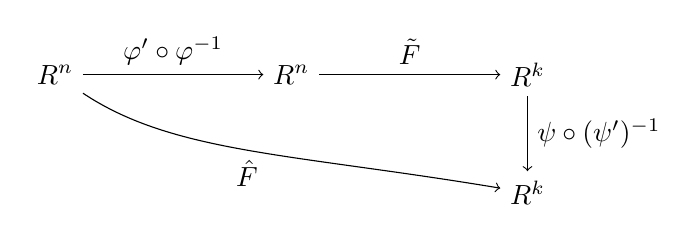
\begin{tikzpicture}[node distance=3cm, auto]
			% Nós
			\node (R1) {$\mathbb{R}^n$};
			\node (R2) [right of=R1] {$\mathbb{R}^n$};
			\node (R3) [right of=R2] {$\mathbb{R}^k$};
			\node (R4) [below of=R3, node distance=1.5cm] {$\mathbb{R}^k$};
			
			% Setas
			\draw[->] (R1) -- node {$\varphi' \circ \varphi^{-1}$} (R2);
			\draw[->] (R2) -- node {$\tilde{F}$} (R3);
			\draw[->] (R3) -- node {$\psi \circ (\psi')^{-1}$} (R4);
			\draw[->] (R1) .. controls (1.5, -1) and (3, -1) .. (R4) node [midway, below] {$\hat{F}$};
		\end{tikzpicture}
		\caption{Diagrama comutativo da representação coordenada.}
	\end{figure}
	
	\textbf{3. Análise da suavidade dos componentes:}
	\begin{itemize}
		\item A aplicação $\varphi' \circ \varphi^{-1}$ é a função de transição entre as cartas $\varphi$ e $\varphi'$ em $M^n$, que é um difeomorfismo, logo é suave.
		\item A aplicação $\tilde{F} = \psi' \circ F \circ (\varphi')^{-1}$ é suave por hipótese, dada a suavidade de $F$.
		\item A aplicação $\psi \circ (\psi')^{-1}$ é a função de transição entre as cartas $\psi'$ e $\psi$ em $N^k$, que é um difeomorfismo, logo é suave.                        
	\end{itemize}
	
	Como $\hat{F}$ é a composição de três aplicações suaves entre abertos de espaços euclidianos, temos que $\hat{F}$ é suave. Como $p$ foi escolhido arbitrariamente, a representação coordenada é suave para qualquer par de cartas suaves.
}
%%%% QUESTÃO 16 %%%%
\questao{
	Mostre que difeomorfismos definem uma relação de equivalência no conjunto de variedades suaves. Além disso, mostre que o conjunto dos difeomorfismos de uma $n$-variedade suave $M^{n}$, munido com a operação da composição, é um grupo.
}
\solucao{
	
	\textbf{Análise do Enunciado}
	\begin{itemize}
		\item \textbf{Hipóteses:} $\mathcal{M}$ é o conjunto de todas as variedades suaves; a relação $\sim$ é definida pela existência de um difeomorfismo entre duas variedades.
		\item \textbf{Tese 1:} Provar que a relação $\sim$ é de equivalência (reflexiva, simétrica e transitiva).
		\item \textbf{Tese 2:} Provar que $\text{Diff}(M^n)$, com a operação de composição, satisfaz os axiomas de grupo.
	\end{itemize}
	\vspace{5pt}
	\textbf{1. Prova da Relação de Equivalência}
	
	Seja $\mathcal{M}$ o conjunto de todas as variedades suaves. Definimos a relação $\sim$ em $\mathcal{M}$ da seguinte forma: para quaisquer variedades suaves $M, N \in \mathcal{M}$, dizemos que $M \sim N$ se, e somente se, existe um difeomorfismo $f: M \to N$. Para que $\sim$ seja uma relação de equivalência, ela deve satisfazer as seguintes propriedades:
	
	\begin{itemize}
		\item \textbf{Reflexividade:} Para qualquer variedade $M$, a aplicação identidade $\text{Id}_M: M \to M$ é um homeomorfismo e é suave (pois a representação coordenada $\text{Id}_{\mathbb{R}^n}$ é suave). Como $(\text{Id}_M)^{-1} = \text{Id}_M$ também é suave, $\text{Id}_M$ é um difeomorfismo. Logo, $M \sim M$.
		
		\item \textbf{Simetria:} Suponha que $M \sim N$. Então existe um difeomorfismo $f: M \to N$. Por definição de difeomorfismo, $f$ é bijetiva e possui uma inversa $f^{-1}: N \to M$ que também é suave. Como $f^{-1}$ é suave e sua inversa $(f^{-1})^{-1} = f$ também é suave, $f^{-1}$ é um difeomorfismo de $N$ para $M$. Logo, $N \sim M$.
		
		\item \textbf{Transitividade:} Suponha que $M \sim N$ e $N \sim L$. Então existem difeomorfismos $f: M \to N$ e $g: N \to L$. Consideremos a composição $g \circ f: M\to P$. 
		Como $f$ e $g$ são bijetivas, $g \circ f$ é bijetiva. A inversa de $g \circ f$ é dada por $(g \circ f)^{-1} = f^{-1} \circ g^{-1}$. 
		Como $f, g, f^{-1}$ e $g^{-1}$ são aplicações suaves, e a composição de aplicações suaves é suave, concluímos que tanto $g \circ f$ quanto $f^{-1} \circ g^{-1}$ são suaves. Portanto, $g \circ f$ é um difeomorfismo de $M$ para $L$, logo $M \sim L$.
	\end{itemize}
	
	Como a relação é reflexiva, simétrica e transitiva, os difeomorfismos definem uma relação de equivalência em $\mathcal{M}$.
	
	\textbf{2. Prova da Estrutura de Grupo de $\text{Diff}(M^n)$}
	
	Seja $\text{Diff}(M^n)$ o conjunto de todos os difeomorfismos de uma $n$-variedade suave $M^n$ para si mesma. Consideremos a operação de composição $\circ$. Verificamos os axiomas de grupo:
	
	\begin{itemize}
		\item \textbf{Fechamento:} Sejam $f, g \in \text{Diff}(M^n)$. Como $f$ e $g$ são difeomorfismos, a composição $f \circ g: M^n \to M^n$ é bijetiva e suave. Sua inversa $(f \circ g)^{-1} = g^{-1} \circ f^{-1}$ também é a composição de difeomorfismos, logo é suave. Portanto, $f \circ g \in \text{Diff}(M^n)$.
		
		\item \textbf{Associatividade:} Para quaisquer $f, g, h \in \text{Diff}(M^n)$ e qualquer $p \in M^n$:
		\begin{equation*}
			(f \circ (g \circ h))(p) = f(g(h(p))) = ((f \circ g) \circ h)(p),
		\end{equation*}
		pois a composição é associativa e composição de difeomorfismos é difeomorfismo.
		
		\item \textbf{Elemento Neutro:} A aplicação identidade $\text{Id}_M: M^n \to M^n$ pertence a $\text{Diff}(M^n)$. Para qualquer $f \in \text{Diff}(M^n)$, temos:
		\begin{equation*}
			f \circ \text{Id}_M = f = \text{Id}_M \circ f.
		\end{equation*}
		
		\item \textbf{Elemento Inverso:} Para qualquer $f \in \text{Diff}(M^n)$, existe por definição a aplicação inversa $f^{-1}: M^n \to M^n$. Como $f$ é um difeomorfismo, $f^{-1}$ também é um difeomorfismo, logo $f^{-1} \in \text{Diff}(M^n)$. Além disso:
		\begin{equation*}
			f \circ f^{-1} = \text{Id}_M = f^{-1} \circ f.
		\end{equation*}
	\end{itemize}
	
	Como todos os axiomas foram satisfeitos,o conjunto $\text{Diff}(M^n)$ munido da composição é um grupo.
}
%%%% QUESTÃO 17 %%%%
\questao{
	Mostre que duas variedades suaves difeomorfas possuem a mesma dimensão.
}
\solucao{
	
	\textbf{Análise do Enunciado}
	\begin{itemize}
		\item \textbf{Hipóteses:} $M$ e $N$ são variedades suaves de dimensões $m$ e $n$, respectivamente, e existe um difeomorfismo $f: M \to N$.
		\item \textbf{Tese:} Provar que $m = n$.
	\end{itemize}
	\vspace{5pt}
	Sejam $M$ e $N$ variedades suaves de dimensões $m$ e $n$, respectivamente. Por hipótese, existe um difeomorfismo $f: M \to N$.
	
	\textbf{1. Representação Coordenada:}
	Seja $p \in M$ e consideremos a representação coordenada $\hat{f} = \psi \circ f \circ \varphi^{-1}$ em relação a cartas suaves $(U, \varphi)$ em $M$ e $(V, \psi)$ em $N$. Como $f$ é um difeomorfismo, $\hat{f}$ é um difeomorfismo entre o aberto $\varphi(U \cap f^{-1}(V)) \subseteq \mathbb{R}^m$ e o aberto $\psi(f(U \cap f^{-1}(V))) \subseteq \mathbb{R}^n$.
	
	\textbf{2. Análise do Diferencial:}
	Para qualquer ponto $x$ no domínio de $\hat{f}$, a aplicação $\hat{f}$ é suave e possui uma inversa suave $\hat{f}^{-1}$. Pela regra da cadeia, a composição $\hat{f}^{-1} \circ \hat{f} = \text{Id}_{\mathbb{R}^m}$ implica que:
	\begin{equation*}
		d(\hat{f}^{-1})_{\hat{f}(x)} \circ d\hat{f}_x = \text{Id}_{\mathbb{R}^m}.
	\end{equation*}
	Analogamente, $\hat{f} \circ \hat{f}^{-1} = \text{Id}_{\mathbb{R}^n}$ implica que:
	\begin{equation*}
		d\hat{f}_x \circ d(\hat{f}^{-1})_{\hat{f}(x)} = \text{Id}_{\mathbb{R}^n}.
	\end{equation*}
	
	\textbf{3. Isomorfismo de Espaços Vetoriais:}
	As equações acima demonstram que o diferencial $d\hat{f}_x : \mathbb{R}^m \to \mathbb{R}^n$ é uma aplicação linear invertível, ou seja, é um isomorfismo de espaços vetoriais. Como a dimensão de um espaço vetorial é preservada por isomorfismos, temos necessariamente que:
	\begin{equation*}
		\dim(\mathbb{R}^m) = \dim(\mathbb{R}^n) \implies m = n.
	\end{equation*}
	Assim, as variedades $M$ e $N$ possuem a mesma dimensão.
}
%%%% QUESTÃO 18 %%%%
\questao{
	Considere variedades suaves $M^{m}$ e $N^{n}$ de dimensão $m$ e $n$, respectivamente. Sejam $\mathcal{U} = \{(U_{i}, \phi_{i})\}_{i \in I}$ e $\mathcal{V} = \{(V_{j}, \psi_{j})\}_{j \in J}$ atlas suaves para $M^{m}$ e $N^{n}$, respectivamente. Mostre que:
	\begin{enumerate}[label=(\alph*)]
		\item $\mathcal{U} \times \mathcal{V} = \{(U_{i} \times V_{j}, \phi_{i} \times \psi_{j})_{i \in I, j \in J}\}$ é um atlas suave em $M^{m} \times N^{n}$.
		\item As projeções $\pi_{1} : M^{m} \times N^{n} \to M^{m}$ e $\pi_{2} : M^{m} \times N^{n} \to N^{n}$ são aplicações suaves.
		\item Se $P^{k}$ é uma outra variedade suave, $g : P^{k} \to M^{m} \times N^{n}$ é suave se, e somente se, $\pi_{i} \circ g$ é suave para todo $i \in \{1,2\}$.
		\item Para $y \in N^{n}$, a aplicação inclusão 
		\begin{eqnarray*}
			\iota : M^{m}& \longrightarrow &M^{m} \times N^{n}\\
			x&\longmapsto& (x,y),
		\end{eqnarray*}
		é suave
		\item $M^{m} \times N^{n}$ é difeomorfo a $N^{n} \times M^{m}$.
	\end{enumerate}
}
\solucao{
	
	\textbf{Análise do Enunciado}
	\begin{itemize}
		\item \textbf{Hipóteses:} $M^m$ e $N^n$ são variedades suaves com atlas $\mathcal{U}$ e $\mathcal{V}$.
		\item \textbf{Tese (a):} Provar que o produto de atlas define uma estrutura suave em $M \times N$.
		\item \textbf{Tese (b):} Provar a suavidade das projeções canônicas $\pi_i$.
		\item \textbf{Tese (c):} Provar a caracterização de suavidade de $g$ via projeções.
		\item \textbf{Tese (d):} Provar que a inclusão de $M$ em $M \times N$ (fixando $y$) é suave.
		\item \textbf{Tese (e):} Provar a existência de um difeomorfismo entre $M \times N$ e $N \times M$.
	\end{itemize}
	\vspace{5pt}
	\textbf{(a) Atlas do Produto}
	
	\textbf{Prova da Cobertura e Estrutura Localmente Euclidiana:}
	
	Primeiro, verificamos que a coleção $\mathcal{U} \times \mathcal{V}$ cobre $M^m \times N^n$. Como $\{U_i\}_{i \in I}$ cobre $M$ e $\{V_j\}_{j \in J}$ cobre $N$, temos:
	\begin{equation*}
		\bigcup_{i \in I, j \in J} (U_i \times V_j) = \left( \bigcup_{i \in I} U_i \right) \times \left( \bigcup_{j \in J} V_j \right) = M^m \times N^n.
	\end{equation*}
	Cada carta $\phi_i \times \psi_j : U_i \times V_j \to \mathbb{R}^{m+n}$ é definida por $(\phi_i \times \psi_j)(p, q) = (\phi_i(p), \psi_j(q))$. Como $\phi_i$ e $\psi_j$ são homeomorfismos sobre abertos de $\mathbb{R}^m$ e $\mathbb{R}^n$, o produto $\phi_i \times \psi_j$ é um homeomorfismo sobre o aberto $\phi_i(U_i) \times \psi_j(V_j) \subseteq \mathbb{R}^{m+n}$.
	
	\textbf{Propriedade de Hausdorff:} Sejam $p = (x_1, y_1)$ e $q = (x_2, y_2)$ pontos distintos em $M^m \times N^n$. Então, ou $x_1 \neq x_2$ ou $y_1 \neq y_2$. Se $x_1 \neq x_2$, como $M^m$ é Hausdorff, existem abertos disjuntos $U_1, U_2 \subset M^m$ tais que $x_1 \in U_1$ e $x_2 \in U_2$. Logo, os conjuntos abertos $U_1 \times N^n$ e $U_2 \times N^n$ são disjuntos em $M^m \times N^n$ e separam $p$ e $q$. O raciocínio é análogo caso $y_1 \neq y_2$. Assim, $M^m \times N^n$ é Hausdorff.
	
	\textbf{Base Enumerável:} Sejam $\mathcal{B}_M = \{U_i\}_{i \in \mathbb{N}}$ e $\mathcal{B}_N = \{V_j\}_{j \in \mathbb{N}}$ bases enumeráveis para $M^m$ e $N^n$, respectivamente. Pela definição de topologia produto, a coleção $\mathcal{B}_{M \times N} = \{ U_i \times V_j : i, j \in \mathbb{N} \}$ constitui uma base para a topologia de $M^m \times N^n$. Como o produto cartesiano $\mathbb{N} \times \mathbb{N}$ é enumerável, a base $\mathcal{B}_{M \times N}$ é enumerável.
	
	\textbf{Suavidade das Transições}
	
	Analisamos a função de transição entre duas cartas $(U_i \times V_j, \phi_i \times \psi_j)$ e $(U_k \times V_l, \phi_k \times \psi_l)$:
	\begin{align*}
		(\phi_k \times \psi_l) \circ (\phi_i \times \psi_j)^{-1}(u, v) &= (\phi_k \times \psi_l)(\phi_i^{-1}(u), \psi_j^{-1}(v)) \\
		&= (\phi_k \circ \phi_i^{-1}(u), \psi_l \circ \psi_j^{-1}(v)).
	\end{align*}
	Como $\phi_k \circ \phi_i^{-1}$ e $\psi_l \circ \psi_j^{-1}$ são funções de transição de atlas suaves, elas são $C^\infty$. Como a aplicação total é definida por componentes suaves, a transição no produto é suave.
	
	Portanto, $M^m \times N^n$ é uma variedade suave de dimensão $m+n$ e $\mathcal{U} \times \mathcal{V}$ é um atlas suave.
	
	\textbf{(b) Suavidade das Projeções}
	
	Analisamos a representação coordenada de $\pi_1$ em relação às cartas $\phi_i \times \psi_j$ e $\phi_i$. Para $(u, v) \in \mathbb{R}^m \times \mathbb{R}^n$:
	\begin{align*}
		\phi_i \circ \pi_1 \circ (\phi_i \times \psi_j)^{-1}(u, v) &= \phi_i(\pi_1(\phi_i^{-1}(u), \psi_j^{-1}(v))) \\
		&= \phi_i(\phi_i^{-1}(u)) = u.
	\end{align*}
	A aplicação $(u, v) \mapsto u$ é a projeção canônica de $\mathbb{R}^{m+n}$ em $\mathbb{R}^m$, que é linear e, portanto, suave. O mesmo raciocínio aplica-se a $\pi_2$.
	
	\textbf{(c) Caracterização da Suavidade de $g$}
	
	$(\implies)$ Se $g: P^k \to M \times N$ é suave, então como $\pi_1$ e $\pi_2$ são suaves (provado acima), as composições $\pi_1 \circ g$ e $\pi_2 \circ g$ são suaves, pois a composição de aplicações suaves é suave.
	
	$(\impliedby)$ Suponha que $g_1 = \pi_1 \circ g$ e $g_2 = \pi_2 \circ g$ sejam suaves. Então $g(p) = (g_1(p), g_2(p))$. Seja $(U, \phi)$ uma carta em $P^k$ e $(U_i \times V_j, \phi_i \times \psi_j)$ uma carta em $M \times N$. A representação coordenada de $g$ é:
	\begin{align*}
		(\phi_i \times \psi_j) \circ g \circ \phi^{-1}(u) &= (\phi_i \circ g_1 \circ \phi^{-1}(u), \psi_j \circ g_2 \circ \phi^{-1}(u)).
	\end{align*}
	Como $g_1$ e $g_2$ são suaves, as representações coordenadas $\phi_i \circ g_1 \circ \phi^{-1}$ e $\psi_j \circ g_2 \circ \phi^{-1}$ são suaves. Como cada componente da representação de $g$ é suave, $g$ é suave.
	
	\textbf{(d) Suavidade da Inclusão $\iota$}
	
	Para um ponto $x \in M^m$ e fixo $y \in N^n$, consideremos a representação coordenada de $\iota$:
	\begin{align*}
		(\phi_i \times \psi_j) \circ \iota \circ \phi_k^{-1}(u) &= (\phi_i \times \psi_j)(\iota(\phi_k^{-1}(u))) \\
		&= (\phi_i \times \psi_j)(\phi_k^{-1}(u), y) \\
		&= (\phi_i \circ \phi_k^{-1}(u), \psi_j(y)).
	\end{align*}
	A primeira componente $\phi_i \circ \phi_k^{-1}$ é uma função de transição suave em $M^m$. A segunda componente $\psi_j(y)$ é uma constante em $\mathbb{R}^n$, logo é suave. Assim, $\iota$ é suave.
	
	\textbf{(e) Difeomorfismo entre $M \times N$ e $N \times M$}
	
	Definimos a aplicação de troca $S: M \times N \to N \times M$ por $S(x, y) = (y, x)$. Claramente $S$ é bijetiva e sua inversa é a própria $S$, logo $S$ é um homeomorfismo.
	
	Analisamos a representação coordenada de $S$ em relação aos atlas produto:
	\begin{align*}
		(\psi_j \times \phi_i) \circ S \circ (\phi_i \times \psi_j)^{-1}(u, v) &= (\psi_j \times \phi_i)(S(\phi_i^{-1}(u), \psi_j^{-1}(v))) \\
		&= (\psi_j \times \phi_i)(\psi_j^{-1}(v), \phi_i^{-1}(u)) \\
		&= (\psi_j(\psi_j^{-1}(v)), \phi_i(\phi_i^{-1}(u))) = (v, u).
	\end{align*}
	A aplicação $(u, v) \mapsto (v, u)$ é uma permutação de coordenadas em $\mathbb{R}^{n+m}$, que é linear e suave. Como $S$ e $S^{-1}$ possuem representações coordenadas suaves, $S$ é um difeomorfismo. Portanto, concluímos que, $M^m \times N^n$ e $N^n \times M^m$ são variedades difeomorfas.
}
%%%% QUESTÃO 19 %%%%
\questao{
	Mostre que a aplicação $F : \mathbb{R}^3 \to \mathbb{R}^6$ definida por $F(x, y, z) = (x^2, y^2, z^2, \sqrt{2}xy, \sqrt{2}xz, \sqrt{2}yz)$ induz uma aplicação $f : \mathbb{S}^2 \to \mathbb{S}^5$.
}
\solucao{
	
	\textbf{Análise do Enunciado}
	\begin{itemize}
		\item \textbf{Hipóteses:} $F$ é uma aplicação de $\mathbb{R}^3$ para $\mathbb{R}^6$.
		\item \textbf{Tese:} Provar que a restrição de $F$ ao domínio $\mathbb{S}^2$ tem imagem contida em $\mathbb{S}^5$.
	\end{itemize}
	\vspace{5pt}
	Para provar que $F$ induz a aplicação $f = F|_{\mathbb{S}^2}$, devemos mostrar que a imagem de qualquer ponto $p = (x, y, z) \in \mathbb{S}^2$ pertence à esfera $\mathbb{S}^5$.
	
	\textbf{1. Verificação da Imagem:}
	Como $p \in \mathbb{S}^2$, temos que $x^2 + y^2 + z^2 = 1$. Calculando a norma euclidiana de $F(p)$ ao quadrado, obtemos:
	\begin{align*}
		\|F(p)\|&=\|F(x, y, z)\|^2 = (x^2)^2 + (y^2)^2 + (z^2)^2 + (\sqrt{2}xy)^2 + (\sqrt{2}xz)^2 + (\sqrt{2}yz)^2 \\
		&= x^4 + y^4 + z^4 + 2x^2y^2 + 2x^2z^2 + 2y^2z^2 \\
		&= (x^2 + y^2 + z^2)^2=(1)^2 = 1,
	\end{align*}
	pois $p \in \mathbb{S}^2$.
	
	Portanto, $F(p) \in \mathbb{S}^5$ para todo $p \in \mathbb{S}^2$, o que valida a existência da aplicação induzida $f$.
	
	\textbf{2. Suavidade:}
	Como $F$ é definida por componentes polinomiais, ela é suave em $\mathbb{R}^3$. Sendo $\mathbb{S}^2$ e $\mathbb{S}^5$ subvariedades suaves, a restrição $f = F|_{\mathbb{S}^2}$ é automaticamente uma aplicação suave entre variedades.	
}
%%%% QUESTÃO 20 %%%%
\questao{
	Mostre que a aplicação $F : \mathbb{R}^3 \to \mathbb{R}^6$ definida por $F(x, y, z) = (x^2, y^2, z^2, \sqrt{2}xy, \sqrt{2}xz, \sqrt{2}yz)$ induz uma aplicação $\bar{f} : \mathbb{RP}^2 \to \mathbb{S}^5$.
}
\solucao{
	
	\textbf{Análise do Enunciado}
	\begin{itemize}
		\item \textbf{Hipóteses:} $F$ é a mesma aplicação da questão anterior.
		\item \textbf{Tese:} Provar que $F$ induz uma aplicação bem definida $\bar{f}$ no espaço projetivo $\mathbb{RP}^2$ com imagem em $\mathbb{S}^5$.
	\end{itemize}
	\vspace{5pt}
	Para que a aplicação $F$ induza uma aplicação $\bar{f}$ no espaço projetivo $\mathbb{RP}^2$, ela deve ser constante sobre cada classe de equivalência da relação $\sim$ em $\mathbb{S}^2$. Como $\mathbb{RP}^2$ é o quociente de $\mathbb{S}^2$ pela identificação $p \sim -p$, a condição necessária e suficiente é que $F(p) = F(-p)$ para todo $p \in \mathbb{S}^2$.
	\begin{figure}[htbp]
		\centering
		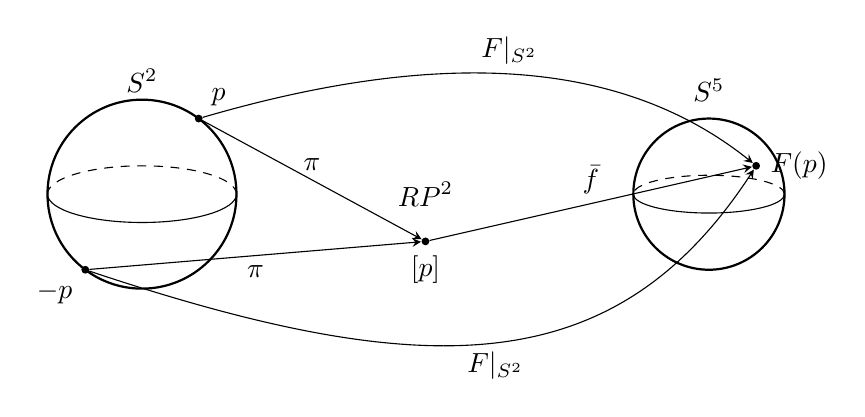
\begin{tikzpicture}[scale=1.2, line join=round, line cap=round]
			\tikzset{
				point/.style={circle, fill=black, inner sep=1pt},
				arrow/.style={->, >=stealth, thin}
			}
			
			% Esfera S2
			\draw[thick] (0,0) circle (1);
			\draw[dashed] (1,0) arc (0:180:1 and 0.3);
			\draw (1,0) arc (0:-180:1 and 0.3);
			\node at (0, 1.2) {$\mathbb{S}^2$};
			
			% Pontos p e -p
			\node[point, label={above right:$p$}] (P) at (0.6, 0.8) {};
			\node[point, label={below left:$-p$}] (mP) at (-0.6, -0.8) {};
			
			% Espaco RP2
			\node (RP) at (3,0) {$\mathbb{RP}^2$};
			\node[point, label={below:$[p]$}] (Proj) at (3, -0.5) {};
			
			% Esfera S5
			\draw[thick] (6,0) circle (0.8);
			\draw[dashed] (6.8,0) arc (0:180:0.8 and 0.2);
			\draw (6.8,0) arc (0:-180:0.8 and 0.2);
			\node at (6, 1.1) {$\mathbb{S}^5$};
			\node[point, label={right:$F(p)$}] (S5) at (6.5, 0.3) {};
			
			% Setas
			\draw[arrow] (P) -- node[midway, above] {$\pi$} (Proj);
			\draw[arrow] (mP) -- node[midway, below] {$\pi$} (Proj);
			\draw[arrow] (Proj) -- node[midway, above] {$\bar{f}$} (S5);
			\draw[arrow] (P) .. controls (3, 1.5) and (5, 1.5) .. (S5) node[midway, above] {$F|_{\mathbb{S}^2}$};
			\draw[arrow] (mP) .. controls (3, -2) and (5, -2) .. (S5) node[midway, below] {$F|_{\mathbb{S}^2}$};
			
		\end{tikzpicture}
		\caption{Diagrama de indução da aplicação $\bar{f}$ via projeção canônica $\pi$.}
	\end{figure}
	\textbf{1. Prova de Boa Definição:}
	Seja $p = (x, y, z) \in \mathbb{S}^2$. O ponto equivalente a $p$ é $-p = (-x, -y, -z)$. Aplicamos $F$ ao ponto $-p$:
	\begin{align*}
		F(-x, -y, -z) &= ((-x)^2, (-y)^2, (-z)^2, \sqrt{2}(-x)(-y), \sqrt{2}(-x)(-z), \sqrt{2}(-y)(-z)) \\
		&= (x^2, y^2, z^2, \sqrt{2}xy, \sqrt{2}xz, \sqrt{2}yz) \\
		&= F(x, y, z).
	\end{align*}
	Como $F(p) = F(-p)$ para qualquer $p \in \mathbb{S}^2$, a aplicação $\bar{f} : \mathbb{RP}^2 \to \mathbb{R}^6$ definida por $\bar{f}([p]) = F(p)$ é bem definida, independentemente do representante escolhido para a classe $[p]$.
	
	\textbf{2. Imagem na Esfera $\mathbb{S}^5$:}
	Conforme provamos na \textbf{Questão 19}, para qualquer $p \in \mathbb{S}^2$, a norma $\|F(p)\|^2 = 1$. Portanto, a imagem de qualquer classe $[p] \in \mathbb{RP}^2$ sob $\bar{f}$ pertence obrigatoriamente à esfera $\mathbb{S}^5$, o que valida o codomínio da aplicação $\bar{f} : \mathbb{RP}^2 \to \mathbb{S}^5$.
	
	\textbf{3. Suavidade:}
	Por construção, temos que $F|_{\mathbb{S}^2} = \bar{f} \circ \pi$, onde $\pi : \mathbb{S}^2 \to \mathbb{RP}^2$ é a projeção canônica. Como $\pi$ é um difeomorfismo local, a suavidade de $\bar{f}$ em um ponto $[p]$ é equivalente à suavidade de $F$ em $p$. Como $F$ é definida por componentes polinomiais, a sua restrição a $\mathbb{S}^2$ é suave. Portanto, a aplicação induzida $\bar{f}$ é suave.
}
%%%% QUESTÃO 21 %%%%
\questao{
	Mostre que a aplicação $F : \mathbb{R}^n \to \mathbb{R}^{\frac{n(n+1)}{2}}$ definida por $$F(x^1, \dots, x^n) = ((x^1)^2, \dots, (x^n)^2, \sqrt{2}x^1x^2, \dots, \sqrt{2}x^{n-1}x^n),$$
	induz uma aplicação $f : \mathbb{S}^{n-1} \to \mathbb{S}^{\frac{n(n+1)}{2}-1}$.
}
\solucao{
	
	\textbf{Análise do Enunciado}
	\begin{itemize}
		\item \textbf{Hipóteses:} $F$ é uma aplicação polinomial de $\mathbb{R}^n$ para $\mathbb{R}^{n(n+1)/2}$.
		\item \textbf{Tese:} Provar que a restrição de $F$ à esfera $\mathbb{S}^{n-1}$ tem imagem contida na esfera de dimensão $\frac{n(n+1)}{2}-1$.
	\end{itemize}
	\vspace{5pt}
	Para provar que $F$ induz a aplicação $f = F|_{\mathbb{S}^{n-1}}$, devemos mostrar que, para qualquer ponto $p = (x^1, \dots, x^n) \in \mathbb{S}^{n-1}$, a norma euclidiana de $F(p)$ é igual a $1$.
	
	\textbf{1. Verificação da Imagem:}
	Como $p \in \mathbb{S}^{n-1}$, as coordenadas de $p$ satisfazem a condição $\sum_{i=1}^n (x^i)^2 = 1$. 
	As componentes de $F(p)$ consistem em $n$ termos do tipo $(x^i)^2$ e $\frac{n(n-1)}{2}$ termos do tipo $\sqrt{2}x^i x^j$ (para $i < j$). Calculamos a norma de $F(p)$ ao quadrado:
	$$\|F(p)\|^2 = \sum_{i=1}^n ((x^i)^2)^2 + \sum_{1 \le i < j \le n} (\sqrt{2}x^i x^j)^2 = \sum_{i=1}^n (x^i)^4 + \sum_{1 \le i < j \le n} 2(x^i)^2(x^j)^2=\left( \sum_{i=1}^n (x^i)^2 \right)^2 = (1)^2 = 1,
	$$
	pois $p \in \mathbb{S}^{n-1}$.
	
	Isso prova que $F(p) \in \mathbb{S}^{\frac{n(n+1)}{2}-1}$ para todo $p \in \mathbb{S}^{n-1}$, validando a existência da aplicação induzida $f$.
	
	\textbf{3. Suavidade:}
	Como $F$ é definida por componentes polinomiais, ela é suave em $\mathbb{R}^n$. Sendo $\mathbb{S}^{n-1}$ e $\mathbb{S}^{\frac{n(n+1)}{2}-1}$ subvariedades suaves, a restrição $f = F|_{\mathbb{S}^{n-1}}$ é automaticamente uma aplicação suave entre variedades.
}
%%%% QUESTÃO 22 %%%%
\questao{
	Para cada $x \in \mathbb{S}^n$ defina $\gamma : \mathbb{R} \to \mathbb{S}^n$ por $\gamma(t) = \cos t \, x + \sen t \frac{v}{\|v\|}$, onde $v \in \mathbb{R}^{n+1} \setminus \{0\}$ é perpendicular a $x$. Mostre que $\gamma$ é suave.
}
\solucao{
	
	\textbf{Análise do Enunciado}
	\begin{itemize}
		\item \textbf{Hipóteses:} $\gamma$ é uma curva parametrizada por $t$ em $\mathbb{R}^{n+1}$, com $x$ e $v/\|v\|$ sendo vetores ortonormais.
		\item \textbf{Tese:} Provar que a imagem de $\gamma$ está em $\mathbb{S}^n$ e que $\gamma$ é uma aplicação suave.
	\end{itemize}
	\vspace{5pt}
	Para provar que $\gamma$ é uma aplicação suave para a esfera $\mathbb{S}^n$, devemos primeiro verificar que a imagem de $\gamma$ está contida em $\mathbb{S}^n$ e, em seguida, analisar a suavidade de suas componentes.
	
	\textbf{1. Verificação da Norma:}
	Seja $u = \frac{v}{\|v\|}$ o vetor unitário na direção de $v$. Por hipótese, $\|x\| = 1$, $\|u\| = 1$ e $x \cdot u = 0$ (pois $v \perp x$). Calculamos a norma de $\gamma(t)$ ao quadrado utilizando o produto escalar:
	\begin{align*}
		\|\gamma(t)\|^2 &= \langle \cos t \, x + \sen t \, u, \cos t \, x + \sen t \, u \rangle \\
		&= \cos^2 t \langle x, x \rangle + \sen^2 t \langle u, u \rangle + 2 \cos t \sen t \langle x, u \rangle \\
		&= \cos^2 t (1) + \sen^2 t (1) + 2 \cos t \sen t (0) \\
		&= \cos^2 t + \sen^2 t = 1.
	\end{align*}
	Como $\|\gamma(t)\| = 1$ para todo $t \in \mathbb{R}$, a imagem de $\gamma$ está contida em $\mathbb{S}^n$, logo a aplicação $\gamma : \mathbb{R} \to \mathbb{S}^n$ está bem definida.
	\begin{figure}[htbp]
		\centering
		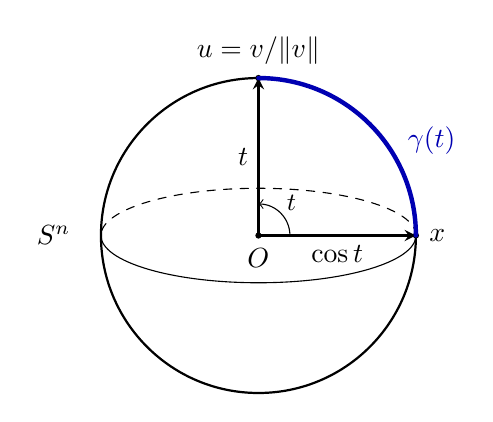
\begin{tikzpicture}[scale=2, line join=round, line cap=round]
			\tikzset{
				point/.style={circle, fill=black, inner sep=0.8pt},
				vector/.style={->, >=stealth, thick}
			}
			
			% Esfera S^n
			\draw[thick] (0,0) circle (1);
			\draw[dashed] (1,0) arc (0:180:1 and 0.3);
			\draw (1,0) arc (0:-180:1 and 0.3);
			\node at (-1.3, 0) {$\mathbb{S}^n$}; % Rótulo na lateral esquerda
			
			% Vetores Ortogonais
			\draw[vector] (0,0) -- (1,0) node[midway, below] {$\cos t$};
			\draw[vector] (0,0) -- (0,1) node[midway, left] {$\sen t$};
			
			% Pontos x e u
			\node[point, label={right:$x$}] (X) at (1,0) {};
			\node[point, label={above:$u = v/\|v\|$}] (U) at (0,1) {};
			\node[point, label={below:$O$} ] at (0,0) {};
			
			% A curva gamma(t)
			\draw[ultra thick, blue!70!black] (1,0) arc (0:90:1);
			\node[blue!70!black] at (1.1, 0.6) {$\gamma(t)$}; % Deslocados para a direita
			
			% Ângulo t - Agora fechando do eixo X ao eixo Y com seta
			\draw[->] (0.2,0) arc (0:90:0.2);
			\node at (0.21, 0.21) {\small $t$};
			
		\end{tikzpicture}
		\caption{Representação da curva $\gamma(t)$ como um círculo máximo no plano gerado por $\{x, u\}$.}
	\end{figure}
	
	\textbf{2. Análise da Suavidade:}
	Consideremos a aplicação $\gamma$ como uma função indo para $\mathbb{R}^{n+1}$. Se denotarmos as componentes de $x$ por $(x^1, \dots, x^{n+1})$ e as de $u$ por $(u^1, \dots, u^{n+1})$, a $i$-ésima componente de $\gamma(t)$ é dada por:
	\begin{equation*}
		\gamma^i(t) = (\cos t)x^i + (\sen t)u^i.
	\end{equation*}
	Como as funções $\sen t$ e $\cos t$ são infinitamente diferenciáveis em $\mathbb{R}$, e $x^i, u^i$ são constantes, cada componente $\gamma^i$ é uma função suave. 
	
	Sendo $\gamma : \mathbb{R} \to \mathbb{R}^{n+1}$ uma aplicação suave e sua imagem contida na subvariedade suave $\mathbb{S}^n$, a aplicação $\gamma : \mathbb{R} \to \mathbb{S}^n$ é, por definição, suave.
}
%%%% QUESTÃO 23 %%%%
\questao{
	Seja $F : \mathbb{R}^{n+1} \to \mathbb{R}^k$ uma aplicação suave. Seja $f = F|_{\mathbb{S}^n}$. Prove que $f$ é suave.
}
\solucao{
	
	\textbf{Análise do Enunciado}
	\begin{itemize}
		\item \textbf{Hipóteses:} $F$ é suave em $\mathbb{R}^{n+1}$. $f$ é a restrição de $F$ à subvariedade $\mathbb{S}^n$.
		\item \textbf{Tese:} Provar que $f: \mathbb{S}^n \to \mathbb{R}^k$ é uma aplicação suave.
	\end{itemize}
	\vspace{5pt}
	Para provar que a restrição $f$ é suave, devemos analisar a estrutura de $f$ como uma composição de aplicações entre variedades suaves.
	
	\textbf{1. Formalização da Restrição via Inclusão:}
	A restrição da aplicação $F$ ao subconjunto $\mathbb{S}^n$ pode ser expressa formalmente através da aplicação de inclusão $\iota : \mathbb{S}^n \hookrightarrow \mathbb{R}^{n+1}$, definida por $\iota(p) = p$ para todo $p \in \mathbb{S}^n$. Assim, a aplicação $f : \mathbb{S}^n \to \mathbb{R}^k$ é dada pela composição:
	\begin{equation*}
		f = F \circ \iota.
	\end{equation*}
	
	\textbf{2. Suavidade da Aplicação de Inclusão:}
	Sabemos que $\mathbb{S}^n$ é uma subvariedade suave de $\mathbb{R}^{n+1}$. Por definição, a aplicação de inclusão $\iota$ é suave se, para qualquer carta $(U, \varphi)$ de $\mathbb{S}^n$, a representação coordenada $\hat{\iota} = \text{Id}_{\mathbb{R}^{n+1}} \circ \iota \circ \varphi^{-1} = \iota \circ \varphi^{-1}$ for suave.
	
	Como $\mathbb{S}^n$ é uma subvariedade suave, a aplicação $\iota \circ \varphi^{-1}$ é, por construção, uma imersão suave de um aberto de $\mathbb{R}^n$ em $\mathbb{R}^{n+1}$. Portanto, $\iota$ é uma aplicação suave.
	
	\textbf{3. Composição de Aplicações Suaves:}
	Temos agora a seguinte sequência de aplicações:
	\begin{equation*}
		\mathbb{S}^n \xrightarrow{\iota} \mathbb{R}^{n+1} \xrightarrow{F} \mathbb{R}^k.
	\end{equation*}
	Como $\iota$ é uma aplicação suave entre a variedade $\mathbb{S}^n$ e a variedade $\mathbb{R}^{n+1}$, e $F$ é uma aplicação suave entre as variedades $\mathbb{R}^{n+1}$ e $\mathbb{R}^k$, a composição $f = F \circ \iota$ é, necessariamente, uma aplicação suave entre as variedades $\mathbb{S}^n$ e $\mathbb{R}^k$.
	
	Como a composição de funções $C^\infty$ preserva a suavidade, concluímos que a restrição $f = F|_{\mathbb{S}^n}$ é suave.
}
%%%% QUESTÃO 24 %%%%	
\questao{
	Seja $F : \mathbb{S}^n \to \mathbb{R}$ uma função suave tal que $F(x) = F(-x)$. Mostre que $F$ induz uma função $\bar{f}$ no espaço projetivo real $\mathbb{RP}^n$ que também é suave.
}
\solucao{
	
	\textbf{Análise do Enunciado}
	\begin{itemize}
		\item \textbf{Hipóteses:} $F$ é suave em $\mathbb{S}^n$ e possui simetria antípoda ($F(x) = F(-x)$).
		\item \textbf{Tese:} Provar que a aplicação induzida $\bar{f}: \mathbb{RP}^n \to \mathbb{R}$ é bem definida e suave.
	\end{itemize}
	\vspace{5pt}
	Consideremos a estrutura de variedade suave de $\mathbb{RP}^n$ estabelecida na \textbf{Questão 4}, onde $\mathbb{RP}^n$ é definido como o quociente de $\mathbb{S}^n$ pela relação $x \sim -x$.
	
	\textbf{1. Boa Definição de $f$:}
	Por hipótese, temos que $F(x) = F(-x)$ para todo $x \in \mathbb{S}^n$. Assim, definimos a função $f : \mathbb{RP}^n \to \mathbb{R}$ da seguinte forma, $f([x]) = F(x)$, onde $[x]$ denota a classe de equivalência $\{x, -x\}$. Como a imagem de $F$ é a mesma para qualquer representante da classe $[x]$, a função $f$ está bem definida.
	
	\textbf{2. Suavidade de $\bar{f}$:}
	Para provar a suavidade de $\bar{f}$, utilizamos as cartas coordenadas $(U_i, \phi_i)$ definidas na \textbf{Questão 4}. Seja $p = [x] \in U_i$, a representação coordenada de $\bar{f}$ é a aplicação $\bar{f} \circ \phi_i^{-1}$ e a aplicação $\phi_i^{-1} : \phi_i(U_i) \to U_i$ pode ser composta com a projeção $\pi : \mathbb{S}^n \to \mathbb{RP}^n$ para obter uma aplicação suave $\sigma_i : \phi_i(U_i) \to \mathbb{S}^n$, tal que $\pi \circ \sigma_i = \phi_i^{-1}$. Assim, a representação de $\bar{f}$ torna-se, $\bar{f} \circ \phi_i^{-1} = \bar{f} \circ (\pi \circ \sigma_i) = (\bar{f} \circ \pi) \circ \sigma_i$. Por outro lado, da definição de $\bar{f}$, temos que $\bar{f} \circ \pi = F$. Portanto, 
	$$\boxed{\bar{f} \circ \phi_i^{-1} = F \circ \sigma_i}$$
	\begin{figure}[htbp]
		\centering
		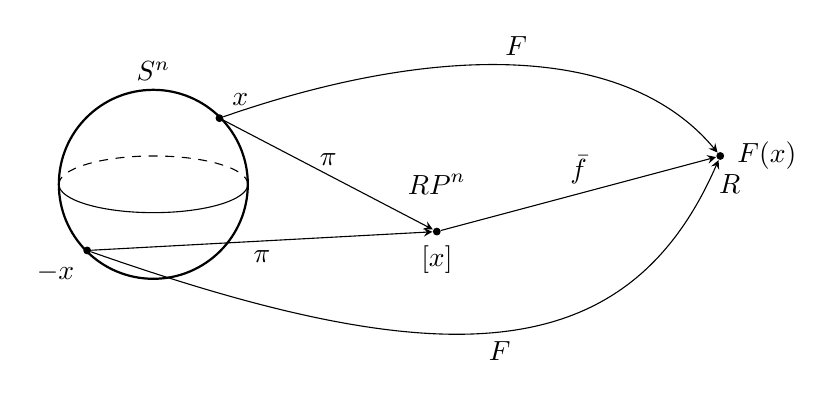
\begin{tikzpicture}[scale=1.2, line join=round, line cap=round]
			\tikzset{
				point/.style={circle, fill=black, inner sep=1pt},
				arrow/.style={->, >=stealth, thin}
			}
			
			% S^n
			\draw[thick] (0,0) circle (1);
			\draw[dashed] (1,0) arc (0:180:1 and 0.3);
			\draw (1,0) arc (0:-180:1 and 0.3);
			\node at (0, 1.2) {$\mathbb{S}^n$};
			
			% Pontos x e -x
			\node[point, label={above right:$x$}] (X) at (0.7, 0.7) {};
			\node[point, label={below left:$-x$}] (mX) at (-0.7, -0.7) {};
			
			% RP^n
			\node (RP) at (3,0) {$\mathbb{RP}^n$};
			\node[point, label={below:$[x]$}] (Proj) at (3, -0.5) {};
			
			% R
			\node (R) at (6.1,0) {$\mathbb{R}$};
			\node[point, label={right, xshift=1pt:$F(x)$}] (Val) at (6, 0.3) {};
			
			% Setas
			\draw[arrow] (X) -- node[midway, above] {$\pi$} (Proj);
			\draw[arrow] (mX) -- node[midway, below] {$\pi$} (Proj);
			\draw[arrow] (Proj) -- node[midway, above] {$\bar{f}$} (Val);
			\draw[arrow] (X) .. controls (3, 1.5) and (5, 1.5) .. (Val) node[midway, above] {$F$};
			\draw[arrow] (mX) .. controls (3, -2) and (5, -2) .. (Val) node[midway, below] {$F$};
			
		\end{tikzpicture}
		\caption{Diagrama de comutação - a função $F$ em $\mathbb{S}^n$ induz a função $\bar{f}$ em $\mathbb{RP}^n$ via projeção $\pi$.}
	\end{figure}
	
	Como $F$ é uma função suave em $\mathbb{S}^n$ e $\sigma_i$ é uma aplicação suave entre abertos de $\mathbb{R}^n$ e $\mathbb{S}^n$, a composição $F \circ \sigma_i$ é suave. Como a representação de $\bar{f}$ em qualquer carta da Questão 4 é suave, concluímos que $\bar{f}$ é uma função suave.
}
%%%% QUESTÃO 25 %%%%
\questao{
	Seja $F : \mathbb{S}^n \to \mathbb{S}^n$ definida por $F(x) = -x$. Mostre que $F$ é um difeomorfismo.
}
\solucao{
	
	\textbf{Análise do Enunciado}
	\begin{itemize}
		\item \textbf{Hipóteses:} $F$ é a aplicação antípoda da esfera $\mathbb{S}^n$ para si mesma.
		\item \textbf{Tese:} Provar que $F$ é um difeomorfismo.
	\end{itemize}
	\vspace{5pt}
	Para provar que $F$ é um difeomorfismo, devemos mostrar que ela é bijetiva e que tanto $F$ quanto sua inversa $F^{-1}$ são aplicações suaves.
	
	\textbf{1. Bijetividade e Inversa:}
	Seja $x \in \mathbb{S}^n$. a aplicação $F$ envia cada ponto ao seu ponto antípoda. Verifiquemos a composição de $F$ com ela mesma:
	\begin{equation*}
		(F \circ F)(x) = F(F(x)) = F(-x) = -(-x) = x.
	\end{equation*}
	Como $F \circ F = \text{Id}_{\mathbb{S}^n}$, a aplicação $F$ é a sua própria inversa ($F = F^{-1}$). Toda aplicação que possui inversa é, necessariamente, bijetiva.
	
	\textbf{2. Suavidade de $F$:}
	Consideremos a aplicação linear $L : \mathbb{R}^{n+1} \to \mathbb{R}^{n+1}$ definida por $L(v) = -v$. Como $L$ é uma aplicação linear, ela é suave em todo o seu domínio $\mathbb{R}^{n+1}$.
	
	A aplicação $F$ é precisamente a restrição de $L$ ao subconjunto $\mathbb{S}^n$:
	\begin{equation*}
		F = L|_{\mathbb{S}^n}.
	\end{equation*}
	Sendo $\mathbb{S}^n$ uma subvariedade suave de $\mathbb{R}^{n+1}$ e $L$ uma aplicação suave no espaço ambiente, a restrição $F$ é, por definição, uma aplicação suave entre variedades.
	
	\textbf{3. Suavidade de $F^{-1}$:}
	Visto que $F^{-1} = F$, a suavidade da inversa é idêntica à suavidade da aplicação original. Portanto, $F^{-1}$ também é suave. Como $F$ é bijetiva, suave e possui inversa suave, concluímos que $F$ é um difeomorfismo da esfera $\mathbb{S}^n$ para si mesma.
}
%%%% QUESTÃO 26 %%%%
\questao{
	Seja $F : \mathbb{R}^{n+1} \setminus \{0\} \to \mathbb{R}^{n+1}$ dada por $F(x) = \frac{x}{|x|}$. Mostre que $F$ é uma função suave e $F(\mathbb{R}^{n+1} \setminus \{0\}) = \mathbb{S}^n$.
}
\solucao{
	
	\textbf{Análise do Enunciado}
	\begin{itemize}
		\item \textbf{Hipóteses:} $F$ é a aplicação de normalização de vetores.
		\item \textbf{Tese 1:} Provar a suavidade de $F$.
		\item \textbf{Tese 2:} Provar que a imagem de $F$ é exatamente a esfera $\mathbb{S}^n$.
	\end{itemize}
	\vspace{5pt}
	\textbf{1. Prova da Suavidade de $F$:}
	Analisamos a suavidade de $F$ examinando a expressão de suas componentes. Para qualquer $x = (x^1, \dots, x^{n+1})$ pertencente ao domínio $\mathbb{R}^{n+1} \setminus \{0\}$, a $i$-ésima componente de $F(x)$ é:
	\begin{equation*}
		F_i(x) = \frac{x^i}{\sqrt{(x^1)^2 + \dots + (x^{n+1})^2}}.
	\end{equation*}
	Para provar que $F_i$ é suave, analisamos a composição de funções:
	\begin{itemize}
		\item A função $g: \mathbb{R}^{n+1} \to \mathbb{R}$ dada por $g(x) = \sum_{j=1}^{n+1} (x^j)^2$ é um polinômio, sendo, portanto, suave em todo $\mathbb{R}^{n+1}$.
		\item A função $\sqrt{\cdot}$ é suave no intervalo $(0, \infty)$. Como o domínio de $F$ é precisamente $\mathbb{R}^{n+1} \setminus \{0\}$, temos que $g(x) > 0$ para todo $x$ no domínio. Assim, a composição $\sqrt{g(x)} = |x|$ é suave em $\mathbb{R}^{n+1} \setminus \{0\}$.
		\item O numerador $x^i$ é uma função linear, logo é suave em $\mathbb{R}^{n+1}$.
	\end{itemize}
	Sendo $F_i$ o quociente de duas funções suaves onde o denominador $|x|$ nunca se anula no domínio $\mathbb{R}^{n+1} \setminus \{0\}$, concluímos que cada componente $F_i$ é suave. Portanto, $F$ é uma aplicação suave no aberto $\mathbb{R}^{n+1} \setminus \{0\}$.
	
	\textbf{2. Prova de que a Imagem é $\mathbb{S}^n$:}
	Para mostrar que $F(\mathbb{R}^{n+1} \setminus \{0\}) = \mathbb{S}^n$, provaremos as duas inclusões:
	
	($\subseteq$) Seja $x \in \mathbb{R}^{n+1} \setminus \{0\}$. Calculamos a norma da imagem $F(x)$:
	\begin{align*}
		\|F(x)\| &= \left\| \frac{1}{|x|} \cdot x \right\| = \frac{1}{|x|} \|x\| = \frac{|x|}{|x|} = 1.
	\end{align*}
	Como a norma de $F(x)$ é igual a $1$, temos que $F(x) \in \mathbb{S}^n$ para todo $x$ no domínio. Logo, $F(\mathbb{R}^{n+1} \setminus \{0\}) \subseteq \mathbb{S}^n$.
	
	($\supseteq$) Seja $y \in \mathbb{S}^n$. Por definição, $\|y\| = 1$. Note que $y \neq 0$, logo $y$ pertence ao domínio de $F$. Calculando a imagem de $y$:
	\begin{align*}
		F(y) = \frac{y}{|y|} = \frac{y}{1} = y.
	\end{align*}
	Isso mostra que qualquer ponto $y \in \mathbb{S}^n$ possui um pré-imaginário no domínio de $F$ (o próprio $y$). Logo, $$\mathbb{S}^n \subseteq F(\mathbb{R}^{n+1} \setminus \{0\}).$$
	
	Tendo provadas as duas inclusões, concluímos que $F(\mathbb{R}^{n+1} \setminus \{0\}) = \mathbb{S}^n$.
}
%%%% QUESTÃO 27 %%%%	
\questao{
Mostre que a aplicação $F : \mathbb{R}^3 \to \mathbb{R}^6$ definida por $F(x, y, z) = (x^2, y^2, z^2, \sqrt{2}xy, \sqrt{2}xz, \sqrt{2}yz)$ induz uma aplicação suave injetiva $f : \mathbb{RP}^2 \to \mathbb{S}^5$.
}
\solucao{
	
	\textbf{Análise do Enunciado}
	\begin{itemize}
		\item \textbf{Hipóteses:} $F$ é a aplicação polinomial dada.
		\item \textbf{Tese:} Provar que $F$ induz uma aplicação $f: \mathbb{RP}^2 \to \mathbb{S}^5$ que seja suave e injetiva.
	\end{itemize}
	\vspace{5pt}
	\textbf{1. Indução e Suavidade:}
	Com base nos resultados das \textbf{Questões 19 e 20}, sabemos que $F(\mathbb{S}^2) \subseteq \mathbb{S}^5$ e $F(x) = F(-x)$ para todo $x \in \mathbb{S}^2$. Portanto, a aplicação $f([x]) = F(x)$ está bem definida e é suave, pois é a descida de uma aplicação suave para um espaço quociente via projeção canônica.
	
	\textbf{2. Prova de Injetividade via Sistema de Equações não Linear:}
	Sejam $[x], [y] \in \mathbb{RP}^2$ dois pontos tais que $f([x]) = f([y])$. Isso implica que, para representantes $x, y \in \mathbb{S}^2$, temos a igualdade $F(x) = F(y)$, o que é equivalente ao seguinte sistema de equações:
	\begin{equation*}
		\begin{cases}
			x_1^2 = y_1^2 \\
			x_2^2 = y_2^2 \\
			x_3^2 = y_3^2 \\
			x_1x_2 = y_1y_2 \\
			x_1x_3 = y_1y_3 \\
			x_2x_3 = y_2y_3
		\end{cases}
	\end{equation*}
	
	Como $x \in \mathbb{S}^2$, temos $\sum x_i^2 = 1$, logo $x \neq 0$. Suponhamos, sem perda de generalidade, que $x_1 \neq 0$. A primeira equação do sistema implica que $y_1 = \pm x_1$.
	
	Analisamos a consistência dos sinais nos dois casos possíveis:
	
	\textbf{Caso 1: $y_1 = x_1$}
	Substituindo $y_1 = x_1$ nas equações de produtos mistos:
	\begin{align*}
		x_1x_2 = y_1y_2 &\implies x_1x_2 = x_1y_2 \implies x_1(x_2 - y_2) = 0 \\
		x_1x_3 = y_1y_3 &\implies x_1x_3 = x_1y_3 \implies x_1(x_3 - y_3) = 0.
	\end{align*}
	Como $x_1 \neq 0$, deduzimos que $y_2 = x_2$ e $y_3 = x_3$. Portanto, $y = x$.
	
	\textbf{Caso 2: $y_1 = -x_1$}
	Substituindo $y_1 = -x_1$ nas equações de produtos mistos:
	\begin{align*}
		x_1x_2 = y_1y_2 &\implies x_1x_2 = -x_1y_2 \implies x_1(x_2 + y_2) = 0 \\
		x_1x_3 = y_1y_3 &\implies x_1x_3 = -x_1y_3 \implies x_1(x_3 + y_3) = 0.
	\end{align*}
	Como $x_1 \neq 0$, deduzimos que $y_2 = -x_2$ e $y_3 = -x_3$. Portanto, $y = -x$.
	
	Em ambos os casos, concluímos que $y = \pm x$. Pela definição de equivalência no espaço projetivo real, isso implica que:
	\begin{equation*}
		[x] = [y].
	\end{equation*}
	
	Como a igualdade das imagens $f([x]) = f([y])$ implica a igualdade dos pontos $[x] = [y]$, a aplicação $f$ é injetiva.
	
	\textbf{2* (alternativa). Prova de Injetividade via Operadores Lineares:}
	Para provar a injetividade, utilizaremos a identificação de $F$ com o espaço de matrizes simétricas $S(3, \mathbb{R})$ discutida na \textbf{Questão 9}. Observemos que a aplicação $F(x)$ representa as componentes da matriz simétrica de posto 1 dada pelo produto externo $A_x = x x^T$. Especificamente:
	\begin{equation*}
		A_x = x x^T = \begin{pmatrix} x_1^2 & x_1x_2 & x_1x_3 \\ x_2x_1 & x_2^2 & x_2x_3 \\ x_3x_1 & x_3x_2 & x_3^2 \end{pmatrix}.
	\end{equation*}
	Sejam $[x], [y] \in \mathbb{RP}^2$ tais que $f([x]) = f([y])$. Isso implica que $F(x) = F(y)$, o que equivale a dizer que as matrizes simétricas associadas são idênticas:
	\begin{equation*}
		x x^T = y y^T.
	\end{equation*}
	Como $x, y \in \mathbb{S}^2$, ambos são vetores não nulos. Para qualquer matriz da forma $v v^T$, a imagem do operador linear é o subespaço unidimensional gerado por $v$. Assim, a igualdade de operadores implica a igualdade de suas imagens:
	\begin{equation*}
		\text{Im}(x x^T) = \text{Im}(y y^T) \implies \text{span}\{x\} = \text{span}\{y\}.
	\end{equation*}
	A igualdade de subespaços unidimensionais implica que $x$ e $y$ são colineares, ou seja, existe $\lambda \in \mathbb{R} \setminus \{0\}$ tal que $y = \lambda x$. Como $\|x\| = 1$ e $\|y\| = 1$, temos que $|\lambda| = 1$, logo $\lambda = \pm 1$.
	
	Portanto, $y = x$ ou $y = -x$. Pela definição de equivalência no espaço projetivo, isso significa que $[x] = [y]$. Assim, a aplicação $f$ é injetiva.
	
	Como $f$ é suave e injetiva, a tese está provada.	
}
%%%% QUESTÃO 28 %%%%
\questao{
	Mostre que a aplicação $F : \mathbb{R}^3 \to \mathbb{R}^5$ definida por $$F(x, y, z) = \left(\sqrt{3}xy, \sqrt{3}xz, \sqrt{3}yz, \frac{\sqrt{3}}{2}(x^2 - y^2), \frac{1}{2}x^2 + \frac{1}{2}y^2 - z^2\right),$$ induz uma aplicação suave injetiva $\bar{f} : \mathbb{RP}^2 \to \mathbb{S}^4$.
}
\solucao{
	\textbf{Análise do Enunciado}
	\begin{itemize}
		\item \textbf{Hipóteses:} $F$ é uma aplicação polinomial de $\mathbb{R}^3$ para $\mathbb{R}^5$.
		\item \textbf{Tese 1:} Provar que $F$ induz uma aplicação bem definida $\bar{f}: \mathbb{RP}^2 \to \mathbb{S}^4$ (isso requer que $F$ seja constante nas fibras de $\pi: \mathbb{S}^2 \to \mathbb{RP}^2$ e que a imagem de $\mathbb{S}^2$ esteja em $\mathbb{S}^4$).
		\item \textbf{Tese 2:} Provar que $\bar{f}$ é suave.
		\item \textbf{Tese 3:} Provar que $\bar{f}$ é injetiva.
	\end{itemize}
	\vspace{5pt}
	\textbf{1. Indução e Suavidade:}
	Para que $F$ induza uma aplicação $\bar{f} : \mathbb{RP}^2 \to \mathbb{R}^5$, ela deve ser constante nas fibras da projeção $\pi : \mathbb{S}^2 \to \mathbb{RP}^2$. Seja $p = (x, y, z) \in \mathbb{S}^2$. Calculamos $F(-p)$:
	\begin{align*}
		F(-x, -y, -z) &= \left(\sqrt{3}(-x)(-y), \sqrt{3}(-x)(-z), \sqrt{3}(-y)(-z), \frac{\sqrt{3}}{2}((-x)^2 - (-y)^2), \frac{1}{2}(-x)^2 + \frac{1}{2}(-y)^2 - (-z)^2\right) \\
		&= \left(\sqrt{3}xy, \sqrt{3}xz, \sqrt{3}yz, \frac{\sqrt{3}}{2}(x^2 - y^2), \frac{1}{2}x^2 + \frac{1}{2}y^2 - z^2\right) = F(x, y, z).
	\end{align*}
	Como $F(x) = F(-x)$, a aplicação $\bar{f}([x]) = F(x)$ está bem definida. Além disso, como $F$ é definida por componentes polinomiais, ela é suave em $\mathbb{R}^3$. Sendo $\mathbb{RP}^2$ e $\mathbb{S}^4$ variedades suaves, a aplicação induzida $\bar{f}$ é suave.
	
	\textbf{2. Verificação da Imagem em $\mathbb{S}^4$:}
	Seja $p = (x, y, z) \in \mathbb{S}^2$, logo $x^2 + y^2 + z^2 = 1$. Calculamos a norma de $F(p)$ ao quadrado:
	\begin{align*}
		\|F(p)\|^2 &= (\sqrt{3}xy)^2 + (\sqrt{3}xz)^2 + (\sqrt{3}yz)^2 + \left(\frac{\sqrt{3}}{2}(x^2 - y^2)\right)^2 + \left(\frac{1}{2}x^2 + \frac{1}{2}y^2 - z^2\right)^2 \\
		&= 3x^2y^2 + 3x^2z^2 + 3y^2z^2 + \frac{3}{4}(x^4 + y^4 - 2x^2y^2) + \left(\frac{1}{4}x^4 + \frac{1}{4}y^4 + z^4 + \frac{1}{2}x^2y^2 - x^2z^2 - y^2z^2\right) \\
		&= \left(\frac{3}{4} + \frac{1}{4}\right)x^4 + \left(\frac{3}{4} + \frac{1}{4}\right)y^4 + z^4 + \left(3 - \frac{3}{2} + \frac{1}{2}\right)x^2y^2 + (3 - 1)x^2z^2 + (3 - 1)y^2z^2 \\
		&= x^4 + y^4 + z^4 + 2x^2y^2 + 2x^2z^2 + 2y^2z^2 \\
		&= (x^2 + y^2 + z^2)^2 = (1)^2 = 1.
	\end{align*}
	Portanto, a imagem de $\bar{f}$ está contida em $\mathbb{S}^4$.
	
	\textbf{3. Prova de Injetividade:}
	Sejam $[x], [y] \in \mathbb{RP}^2$ tais que $\bar{f}([x]) = \bar{f}([y])$. Isso implica que $F(x) = F(y)$, resultando no sistema:
	\begin{equation*}
		\begin{cases}
			\sqrt{3}x_1x_2 = \sqrt{3}y_1y_2 \implies x_1x_2 = y_1y_2 \\
			\sqrt{3}x_1x_3 = \sqrt{3}y_1y_3 \implies x_1x_3 = y_1y_3 \\
			\sqrt{3}x_2x_3 = \sqrt{3}y_2y_3 \implies x_2x_3 = y_2y_3 \\
			\frac{\sqrt{3}}{2}(x_1^2 - x_2^2) = \frac{\sqrt{3}}{2}(y_1^2 - y_2^2) \implies x_1^2 - x_2^2 = y_1^2 - y_2^2 \\
			\frac{1}{2}x_1^2 + \frac{1}{2}x_2^2 - x_3^2 = \frac{1}{2}y_1^2 + \frac{1}{2}y_2^2 - y_3^2
		\end{cases}
	\end{equation*}
	Da última equação, e sabendo que $x_1^2 + x_2^2 = 1 - x_3^2$ e $y_1^2 + y_2^2 = 1 - y_3^2$, temos:
	\begin{equation*}
		\frac{1}{2}(1 - x_3^2) - x_3^2 = \frac{1}{2}(1 - y_3^2) - y_3^2 \implies \frac{1}{2} - \frac{3}{2}x_3^2 = \frac{1}{2} - \frac{3}{2}y_3^2 \implies x_3^2 = y_3^2.
	\end{equation*}
	Se $x_3^2 = y_3^2$, então $x_1^2 + x_2^2 = y_1^2 + y_2^2$. Combinando isso com a equação $x_1^2 - x_2^2 = y_1^2 - y_2^2$ através de soma e subtração, obtemos:
	\begin{equation*}
		2x_1^2 = 2y_1^2 \implies x_1^2 = y_1^2 \quad \text{e} \quad 2x_2^2 = 2y_2^2 \implies x_2^2 = y_2^2.
	\end{equation*}
	Agora temos o mesmo sistema da \textbf{Questão 27}: $x_i^2 = y_i^2$ para todo $i$ e $x_i x_j = y_i y_j$ para $i \neq j$. Como demonstrado anteriormente, esse sistema implica necessariamente que $y = x$ ou $y = -x$.
	
	Assim, $[x] = [y]$, o que prova que $\bar{f}$ é injetiva.
}
%%%% RESULTADO EXTRA %%%%
Antes de continuarmos para as próximas questões, é importante estabelecer um resultado fundamental, a saber:
	
\resultadoextra{Teorema da Partição da Unidade.}{
	Seja $M$ uma variedade suave e $\{U_\alpha\}_{\alpha \in \Lambda}$ uma cobertura aberta de $M$. Existe uma família de funções suaves $\{\rho_i\}_{i \in I}$ tal que:
	\begin{enumerate}[label=(\roman*)]
		\item $0 \le \rho_i(p) \le 1$ para todo $p \in M$ e todo $i \in I$.
		\item O suporte de cada $\rho_i$ é compacto e $\text{supp}(\rho_i) \subset U_\alpha$ para algum $\alpha \in \Lambda$.
		\item A família $\{\text{supp}(\rho_i)\}_{i \in I}$ é localmente finita.
		\item $\sum_{i \in I} \rho_i(p) = 1$ para todo $p \in M$.
	\end{enumerate}
}
\solucao{
	
	\textbf{Análise do Enunciado}
	\begin{itemize}
		\item \textbf{Hipóteses:} $M$ é uma variedade suave e $\{U_\alpha\}$ é uma cobertura aberta.
		\item \textbf{Tese:} Provar a existência de uma família de funções suaves com suporte compacto, localmente finita, subordinada à cobertura e com soma unitária.
	\end{itemize}
	\vspace{5pt}
	A demonstração exige a construção de funções suaves com suporte compacto, a refinação da cobertura e a normalização global.
	
	\textbf{1. Construção de Funções Suaves com Suporte Compacto em $\mathbb{R}^n$:}
	Consideremos a função $\psi : \mathbb{R} \to \mathbb{R}$ definida por:
	\begin{equation*}
		\psi(t) = \begin{cases} e^{-1/t} & \text{se } t > 0 \\ 0 & \text{se } t \le 0 \end{cases}
	\end{equation*}
	É um resultado clássico de análise que $\psi$ é suave ($C^\infty$) em todo $\mathbb{R}$, incluindo $t=0$, onde todas as derivadas são nulas. A partir de $\psi$, definimos a função de transição $\eta : \mathbb{R} \to [0, 1]$:
	\begin{equation*}
		\eta(t) = \frac{\psi(t)}{\psi(t) + \psi(1-t)}.
	\end{equation*}
	Note que $\eta(t) = 0$ para $t \le 0$ e $\eta(t) = 1$ para $t \ge 1$. Para qualquer bola aberta $B(x, r) \subset \mathbb{R}^n$, podemos definir uma função suave $\phi_B : \mathbb{R}^n \to [0, 1]$ que é $1$ em $B(x, r/2)$ e $0$ fora de $B(x, r)$, utilizando a composição de $\eta$ com a norma euclidiana:
	\begin{equation*}
		\phi_B(y) = \eta\left( \frac{r/2 - |y-x|}{r/2} \right).
	\end{equation*}
	
	\textbf{2. Refinação da Cobertura e Local Finitude:}
	Como $M$ é uma variedade suave, ela é paracompacta. Portanto, para a cobertura $\{U_\alpha\}$, existe um refinamento aberto $\{V_i\}_{i \in I}$ que é localmente finito e tal que cada $\overline{V}_i$ é compacto e $\overline{V}_i \subset U_\alpha$ para algum $\alpha$. 
	
	Para cada $V_i$, escolhemos uma carta coordenada $(W_i, \varphi_i)$ tal que $V_i \subset W_i$ e a imagem $\varphi_i(V_i)$ seja um aberto em $\mathbb{R}^n$. Podemos então construir, via a função $\phi_B$ definida anteriormente, uma função suave $\psi_i : M \to [0, \infty)$ tal que:
	\begin{itemize}
		\item $\text{supp}(\psi_i) \subset V_i$ (consequentemente, o suporte é compacto e contido em algum $U_\alpha$).
		\item $\psi_i(p) > 0$ para todo $p \in \text{int}(V_i)$.
	\end{itemize}
	
	\textbf{3. Normalização Global:}
	Seja $\Phi : M \to \mathbb{R}$ a soma de todas as funções $\psi_i$:
	\begin{equation*}
		\Phi(p) = \sum_{i \in I} \psi_i(p).
	\end{equation*}
	Como a família $\{\text{supp}(\psi_i)\}$ é localmente finita, para qualquer $p \in M$ existe uma vizinhança onde apenas um número finito de termos da soma é não nulo. Como cada $\psi_i$ é suave, $\Phi$ é suave. Além disso, como $\{V_i\}$ cobre $M$, para cada $p$ existe ao menos um $i$ tal que $\psi_i(p) > 0$, logo $\Phi(p) > 0$ para todo $p \in M$.
	
	Definimos agora as funções $\rho_i : M \to [0, 1]$ por:
	\begin{equation*}
		\rho_i(p) = \frac{\psi_i(p)}{\Phi(p)}.
	\end{equation*}
	
	\textbf{4. Verificação dos Axiomas:}
	\begin{itemize}
		\item \textbf{Suavidade:} $\rho_i$ é o quociente de duas funções suaves com denominador nunca nulo, portanto $\rho_i$ é suave.
		\item \textbf{Suporte:} Como $\text{supp}(\rho_i) = \text{supp}(\psi_i)$, o suporte de $\rho_i$ é compacto e $\text{supp}(\rho_i) \subset U_\alpha$ para algum $\alpha$.
		\item \textbf{Local Finitude:} A local finitude de $\{\rho_i\}$ decorre diretamente da local finitude de $\{\psi_i\}$.
		\item \textbf{Soma Unitária:} Para qualquer $p \in M$:
		\begin{equation*}
			\sum_{i \in I} \rho_i(p) = \sum_{i \in I} \frac{\psi_i(p)}{\Phi(p)} = \frac{1}{\Phi(p)} \sum_{i \in I} \psi_i(p) = \frac{\Phi(p)}{\Phi(p)} = 1.
		\end{equation*}
	\end{itemize}
	
	Assim, concluímos que toda a estrutura necessária para a partição da unidade foi construída.
}
%%%% DEFINIÇÃO %%%%	
\textbf{Definição.} Sejam $M^n$ e $N^k$ variedades suaves e $A \subset M^n$ um subconjunto qualquer. Dizemos que uma função $F : A \to N^k$ é suave se para cada $p \in A$ existe um conjunto aberto $W \subset M^n$ contendo $p$ e uma aplicação suave $\tilde{F} : W \to N^k$ tal que $\tilde{F}|_{W \cap A} = F$.
%%%% QUESTÃO 29 %%%%
\questao{
	\textbf{(Lema de Extensão)} Sejam $M^n$ uma $n$-variedade suave, $A \subset M^n$ um subconjunto fechado e $f : A \to \mathbb{R}^k$ uma função suave. Para qualquer conjunto aberto $U$ contendo $A$, mostre que existe uma função suave $\tilde{f} : M^n \to \mathbb{R}^k$ tal que $\tilde{f}|_A = f$ e $\text{supp } \tilde{f} \subset U$.
}
\solucao{
	
	\textbf{Análise do Enunciado}
	\begin{itemize}
		\item \textbf{Hipóteses:} $A$ é um subconjunto fechado de $M^n$, $f$ é suave em $A$, e $U$ é um aberto tal que $A \subset U$.
		\item \textbf{Tese:} Provar a existência de uma extensão suave $\tilde{f}$ para todo $M^n$ com suporte contido em $U$.
	\end{itemize}
	\vspace{5pt}
	\textbf{1. Construção da Cobertura:}
	Pela definição de suavidade em subconjuntos, para cada $p \in A$, existe um aberto $W_p \subset M^n$ e uma extensão suave $f_p : W_p \to \mathbb{R}^k$ tal que $f_p|_{W_p \cap A} = f$. Definimos $W'_p = W_p \cap U$, garantindo que cada $W'_p$ seja um aberto contendo $p$ e esteja contido em $U$. A coleção $\mathcal{W} = \{W'_p\}_{p \in A} \cup \{M^n \setminus A\}$ constitui uma cobertura aberta de $M^n$.
	
	\textbf{2. Aplicação da Partição da Unidade:}
	Pelo Teorema da Partição da Unidade, existe uma família de funções suaves $\{\rho_i\}_{i \in I}$ subordinada a $\mathcal{W}$. Para cada $\rho_i$, associamos a função $f_i$:
	\begin{itemize}
		\item Se $\text{supp}(\rho_i) \subset W'_p$, definimos $f_i = f_p$.
		\item Se $\text{supp}(\rho_i) \subset M^n \setminus A$, definimos $f_i \equiv 0$.
	\end{itemize}
	Definimos a extensão global $\tilde{f} : M^n \to \mathbb{R}^k$ pela soma localmente finita:
	\begin{equation*}
		\tilde{f}(q) = \sum_{i \in I} \rho_i(q) f_i(q).
	\end{equation*}
	
	\textbf{3. Verificação das Propriedades:}
	Como a soma é localmente finita e cada termo é suave, $\tilde{f}$ é suave. Para qualquer $q \in A$, a função $\rho_i$ associada ao aberto $M^n \setminus A$ é nula, e para todas as demais, $f_i(q) = f(q)$, logo:
	\begin{equation*}
		\tilde{f}(q) = \sum \rho_i(q) f(q) = f(q) \sum \rho_i(q) = f(q).
	\end{equation*}
	Finalmente, se $q \notin U$, então $\rho_i(q) = 0$ para todos os índices onde $f_i \neq 0$ (pois tais suportes estão em $W'_p \subset U$), implicando $\tilde{f}(q) = 0$. Portanto, $\text{supp } \tilde{f} \subset U$.
}
%%%% DEFINIÇÃO %%%%
\textbf{Definição.} Se $M$ é um espaço topológico, uma função de exaustão para $M$ é uma função contínua $f : M \to \mathbb{R}$ tal que o conjunto $M_c = \{x \in M : f(x) \le c\}$ é compacto para cada $c \in \mathbb{R}$.
%%%% QUESTÃO 30 %%%%	
\questao{
	\textbf{(Existência de Funções de Exaustão)} Mostre que qualquer variedade suave admite uma função de exaustão positiva suave.
}
\solucao{
	
	\textbf{Análise do Enunciado}
	\begin{itemize}
		\item \textbf{Hipóteses:} $M$ é uma variedade suave.
		\item \textbf{Tese:} Provar a existência de uma função $f: M \to \mathbb{R}$ que seja suave, positiva e tal que as subníveis $M_c$ sejam compactos.
	\end{itemize}
	\vspace{5pt}
	\textbf{1. Definição e a Propriedade de $\sigma$-compacticidade:}
	Dizemos que um espaço topológico $M$ é $\sigma$-compacto se existe uma família enumerável de subconjuntos compactos $\{K_i\}_{i \in \mathbb{N}}$ tal que $M = \bigcup_{i=1}^\infty K_i$. Como toda variedade suave é, por definição, de Hausdorff e possui base enumerável, ela é necessariamente $\sigma$-compacta.
	
	A partir disso, podemos construir uma \textbf{exaustão por compactos} para $M$. Esta é uma sequência de conjuntos compactos $\{K_i\}_{i=1}^\infty$ tal que:
	\begin{equation*}
		K_1 \subset \text{int}(K_2) \subset K_2 \subset \text{int}(K_3) \subset K_3 \subset \dots \quad \text{e} \quad \bigcup_{i=1}^\infty K_i = M.
	\end{equation*}
	
	\textbf{2. Construção da Função via Partição da Unidade:}
	Para cada $i \ge 1$, definimos o aberto $W_i = \text{int}(K_{i+1}) \setminus K_{i-1}$ (adotando $K_0 = \emptyset$). A coleção $\{W_i\}_{i=1}^\infty$ constitui uma cobertura aberta de $M$. Pelo Teorema da Partição da Unidade, existe uma família de funções suaves $\rho_i : M \to [0, 1]$ tal que $\text{supp}(\rho_i) \subset W_i$ e $\sum_{i=1}^\infty \rho_i(x) = 1$ para todo $x \in M$.
	
	Definimos a função $f : M \to \mathbb{R}$ por:
	\begin{equation*}
		f(x) = \sum_{i=1}^\infty i \cdot \rho_i(x).
	\end{equation*}
	
	\textbf{3. Análise de Suavidade e Positividade:}
	Como a família $\{\text{supp}(\rho_i)\}$ é localmente finita, para qualquer $x \in M$ existe uma vizinhança onde apenas um número finito de termos $\rho_i$ é não nulo. Sendo cada termo $i \cdot \rho_i$ suave, a soma $f$ é suave. Além disso, como $\rho_i(x) \ge 0$ e $\sum \rho_i = 1$, temos $f(x) \ge 1 \cdot \sum \rho_i(x) = 1$. Logo, $f$ é estritamente positiva.
	
	\textbf{4. Prova Algébrica da Propriedade de Exaustão:}
	Seja $c \in \mathbb{R}$ um valor qualquer. Queremos provar que o conjunto $M_c = \{x \in M : f(x) \le c\}$ é compacto. 
	
	Escolhemos um inteiro $N \in \mathbb{N}$ tal que $N > c$. Consideremos agora qualquer ponto $x \in M$ que esteja fora do compacto $K_N$, ou seja, $x \in M \setminus K_N$. 
	
	Para tal ponto $x$, as funções $\rho_i$ com $i < N$ devem ser nulas. De fato, para $i < N$, temos $\text{supp}(\rho_i) \subset \text{int}(K_{i+1}) \subseteq K_N$. Como $x \notin K_N$, segue que $\rho_i(x) = 0$ para todo $i \in \{1, 2, \dots, N-1\}$. 
	
	Calculamos então o valor de $f(x)$ para $x \notin K_N$:
	\begin{align*}
		f(x) &= \sum_{i=1}^\infty i \cdot \rho_i(x) \\
		&= \sum_{i=1}^{N-1} i \cdot 0 + \sum_{i=N}^\infty i \cdot \rho_i(x) \\
		&= \sum_{i=N}^\infty i \cdot \rho_i(x) \ge N \sum_{i=N}^\infty \rho_i(x).
	\end{align*}
	Como $\sum_{i=1}^\infty \rho_i(x) = 1$ e $\rho_i(x) = 0$ para $i < N$, temos que $\sum_{i=N}^\infty \rho_i(x) = 1$. Portanto:
	\begin{equation*}
		f(x) \ge N \cdot 1 = N.
	\end{equation*}
	Dado que escolhemos $N > c$, temos que para todo $x \notin K_N$, $f(x) > c$. 
	
	Isso implica que se $f(x) \le c$, então necessariamente $x \in K_N$. Em termos de conjuntos:
	\begin{equation*}
		M_c \subseteq K_N.
	\end{equation*}
	Como $f$ é contínua, $M_c = f^{-1}((-\infty, c])$ é um subconjunto fechado de $M$. Sendo $M_c$ um fechado contido em um compacto $K_N$, o conjunto $M_c$ é, por consequência, compacto.
	
	Assim, $f$ é uma função de exaustão positiva e suave.
}
%%%% QUESTÃO 31 %%%%
\questao{
	Seja $G$ uma variedade suave munida com uma estrutura de grupo tal que a aplicação $G \times G \to G$, $(g, h) \mapsto gh^{-1}$, é suave. Mostre que $G$ é um grupo de Lie.
}
\solucao{
	
	\textbf{Análise do Enunciado}
	\begin{itemize}
		\item \textbf{Hipóteses:} $G$ é uma variedade suave e um grupo onde a operação combinada $(g,h) \mapsto gh^{-1}$ é suave.
		\item \textbf{Tese:} Provar que $G$ é um grupo de Lie (ou seja, que a multiplicação $m$ e a inversão $i$ são suavemente separadas).
	\end{itemize}
	\vspace{5pt}
	Para provar que $G$ é um grupo de Lie, devemos demonstrar que tanto a aplicação de inversão quanto a aplicação de multiplicação são suaves. Seja $\Phi : G \times G \to G$ a aplicação dada por $\Phi(g, h) = gh^{-1}$, que, por hipótese, é suave.
	
	\textbf{1. Suavidade da Aplicação de Inversão:}
	Consideremos a aplicação de inversão $i : G \to G$ definida por $i(g) = g^{-1}$. 
	Seja $e \in G$ o elemento neutro do grupo. Podemos expressar a aplicação de inversão como uma restrição da aplicação $\Phi$. Fixando o primeiro argumento de $\Phi$ como o elemento neutro $e$, obtemos:
	\begin{equation*}
		\Phi(e, g) = eg^{-1} = g^{-1} = i(g).
	\end{equation*}
	Como $\Phi$ é suave em $G \times G$, a aplicação obtida ao fixar uma das coordenadas (uma aplicação de inclusão $g \mapsto (e, g)$ seguida de $\Phi$) é necessariamente suave. Portanto, a aplicação de inversão $i : G \to G$ é suave.
	
	\textbf{2. Suavidade da Aplicação de Multiplicação:}
	Agora, consideremos a aplicação de multiplicação $m : G \times G \to G$ definida por $m(g, h) = gh$. 
	Podemos expressar a operação de multiplicação utilizando a aplicação $\Phi$ e a aplicação de inversão $i$ que acabamos de provar ser suave. Note que:
	\begin{equation*}
		gh = g(h^{-1})^{-1}.
	\end{equation*}
	Formalmente, definimos a aplicação $\Psi : G \times G \to G \times G$ por $\Psi(g, h) = (g, i(h)) = (g, h^{-1})$. Como $i$ é suave, a aplicação $\Psi$ é suave (pois cada componente é suave). 
	
	A aplicação de multiplicação $m$ pode então ser escrita como a composição:
	\begin{equation*}
		m = \Phi \circ \Psi.
	\end{equation*}
	De fato, para quaisquer $g, h \in G$:
	\begin{align*}
		(\Phi \circ \Psi)(g, h) &= \Phi(\Psi(g, h)) \\
		&= \Phi(g, h^{-1}) \\
		&= g(h^{-1})^{-1} \\
		&= gh.
	\end{align*}
	Como $\Psi$ é suave e $\Phi$ é suave, a composição $\Phi \circ \Psi$ é, necessariamente, suave. Portanto, a aplicação de multiplicação $m$ é suave.
	
	Como a multiplicação e a inversão são aplicações suaves, $G$ satisfaz a definição de um Grupo de Lie.
}
%%%% QUESTÃO 32 %%%%
\questao{
	Mostre que $GL(n, \mathbb{R}) = \{ A \in M(n, \mathbb{R}) : \det A \neq 0 \}$, com a multiplicação usual de matrizes, é um grupo de Lie.
}
\solucao{
	
	\textbf{Análise do Enunciado}
	\begin{itemize}
		\item \textbf{Hipóteses:} $GL(n, \mathbb{R})$ definido como o subconjunto de matrizes invertíveis de $M(n, \mathbb{R})$.
		\item \textbf{Tese:} Provar que $GL(n, \mathbb{R})$ é um grupo de Lie.
	\end{itemize}
	\vspace{5pt}
	\textbf{1. Estrutura de Variedade Suave:}
	Conforme provado na \textbf{Questão 8}, o grupo linear geral $GL(n, \mathbb{R})$ é um subconjunto aberto do espaço de matrizes $M(n, \mathbb{R}) \cong \mathbb{R}^{n^2}$, o que garante que ele seja uma variedade suave de dimensão $n^2$.
	
	\textbf{2. Suavidade da Multiplicação:}
	Seja $m : GL(n, \mathbb{R}) \times GL(n, \mathbb{R}) \to GL(n, \mathbb{R})$ a aplicação de multiplicação $m(A, B) = AB$. A componente $(i, j)$ do produto $AB$ é dada por:
	\begin{equation*}
		(AB)_{ij} = \sum_{k=1}^n A_{ik} B_{kj}.
	\end{equation*}
	Como cada componente $(AB)_{ij}$ é um polinômio nas entradas de $A$ e $B$, a aplicação $m$ é infinitamente diferenciável. Portanto, a multiplicação é suave.
	
	\textbf{3. Suavidade da Inversão:}
	Seja $i : GL(n, \mathbb{R}) \to GL(n, \mathbb{R})$ a aplicação de inversão $i(A) = A^{-1}$. Pela Regra de Cramer, as componentes da matriz inversa são dadas por:
	\begin{equation*}
		(A^{-1})_{ij} = \frac{1}{\det A} (\text{adj } A)_{ji},
	\end{equation*}
	onde $(\text{adj } A)_{ji}$ é o cofator correspondente, que é um polinômio nas entradas de $A$.
	
	Visto que o determinante $\det A$ é uma função suave e nunca se anula no domínio $GL(n, \mathbb{R})$, cada componente $(A^{-1})_{ij}$ é o quociente de duas funções suaves com denominador não nulo. Assim, a aplicação de inversão $i$ é suave.
	
	Tendo sido estabelecida a estrutura de variedade suave e a suavidade das operações de grupo, concluímos que $GL(n, \mathbb{R})$ é um grupo de Lie.
}
%%%% QUESTÃO 33 %%%%
\questao{
	Mostre que $SL(n, \mathbb{R}) = \{ A \in M(n, \mathbb{R}) : \det A = 1 \}$, com a multiplicação usual de matrizes, é um grupo de Lie.
}
\solucao{
	
	\textbf{Análise do Enunciado}
	\begin{itemize}
		\item \textbf{Hipóteses:} $SL(n, \mathbb{R})$ é o subconjunto de matrizes com determinante unitário.
		\item \textbf{Tese:} Provar que $SL(n, \mathbb{R})$ é um grupo de Lie.
	\end{itemize}
	\vspace{5pt}
	\textbf{1. Estrutura de Variedade Suave:}
	Conforme prov도 na \textbf{Questão 10}, a aplicação determinante $\det : M(n, \mathbb{R}) \to \mathbb{R}$ possui o valor $1$ como um valor regular. Pelo Teorema do Valor Regular, o conjunto nível $SL(n, \mathbb{R}) = \det^{-1}(1)$ é uma subvariedade suave de $M(n, \mathbb{R})$ de dimensão $n^2 - 1$.
	
	\textbf{2. Verificação da Estrutura de Subgrupo:}
	Para que $SL(n, \mathbb{R})$ seja um grupo de Lie, as operações de grupo devem estar bem definidas dentro do conjunto. Seja $A, B \in SL(n, \mathbb{R})$, logo $\det A = 1$ e $\det B = 1$.
	
	Pela propriedade multiplicativa do determinante:
	\begin{equation*}
		\det(AB) = \det(A) \cdot \det(B) = 1 \cdot 1 = 1.
	\end{equation*}
	Assim, $AB \in SL(n, \mathbb{R})$, provando que o conjunto é fechado sob a multiplicação. Para a inversão, temos:
	\begin{equation*}
		\det(A^{-1}) = \frac{1}{\det A} = \frac{1}{1} = 1.
	\end{equation*}
	Assim, $A^{-1} \in SL(n, \mathbb{R})$, provando que o conjunto é fechado sob a inversão. Portanto, $SL(n, \mathbb{R})$ é um subgrupo de $GL(n, \mathbb{R})$.
	
	\textbf{3. Suavidade das Operações:}
	Seja $m : GL(n, \mathbb{R}) \times GL(n, \mathbb{R}) \to GL(n, \mathbb{R})$ a aplicação de multiplicação e $i : GL(n, \mathbb{R}) \to GL(n, \mathbb{R})$ a aplicação de inversão. Na \textbf{Questão 32}, provamos que $m$ e $i$ são aplicações suaves.
	
	Como $SL(n, \mathbb{R})$ é uma subvariedade suave de $GL(n, \mathbb{R})$, a restrição da aplicação de multiplicação $m|_{SL \times SL}$ e a restrição da aplicação de inversão $i|_{SL}$ são, por definição, aplicações suaves entre as respectivas variedades.
	
	Como $SL(n, \mathbb{R})$ é uma variedade suave e suas operações de grupo são suaves, concluímos que $SL(n, \mathbb{R})$ é um grupo de Lie.
}
%%%% QUESTÃO 34 %%%%
\questao{
	Mostre que $O(n, \mathbb{R}) = \{ A \in M(n, \mathbb{R}) : AA^T = I \}$, com a multiplicação usual de matrizes, é um grupo de Lie.
}
\solucao{
	
	\textbf{Análise do Enunciado}
	\begin{itemize}
		\item \textbf{Hipóteses:} $O(n, \mathbb{R})$ é o conjunto das matrizes ortogonais.
		\item \textbf{Tese:} Provar que $O(n, \mathbb{R})$ é um grupo de Lie.
	\end{itemize}
	\vspace{5pt}
	\textbf{1. Estrutura de Variedade Suave:}
	Conforme provado detalhadamente na \textbf{Questão 9}, definimos a aplicação $F : M(n, \mathbb{R}) \to S(n, \mathbb{R})$ por $F(A) = AA^T$. Provamos que a identidade $I$ é um valor regular de $F$, o que, pelo Teorema do Valor Regular, implica que o grupo ortogonal $O(n) = F^{-1}(I)$ é uma subvariedade suave de $M(n, \mathbb{R})$ de dimensão $\frac{n(n-1)}{2}$.
	
	\textbf{2. Verificação da Estrutura de Subgrupo:}
	Para que $O(n)$ seja um grupo de Lie, as operações de grupo devem estar bem definidas dentro do conjunto. Sejam $A, B \in O(n)$, logo $AA^T = I$ e $BB^T = I$.
	
	Verifiquemos a multiplicação:
	\begin{equation*}
		(AB)(AB)^T = ABB^T A^T = A I A^T = AA^T = I.
	\end{equation*}
	Assim, $AB \in O(n)$, provando que o conjunto é fechado sob a multiplicação. Para a inversão, note que se $AA^T = I$, então a inversa de $A$ é precisamente a sua transposta, $A^{-1} = A^T$. Verificamos:
	\begin{equation*}
		(A^{-1})(A^{-1})^T = A^T (A^T)^T = A^T A.
	\end{equation*}
	Como $AA^T = I$, a matriz $A$ é invertível e $A^T = A^{-1}$, o que implica que $A^T A = I$. Logo, $A^{-1} \in O(n)$, provando que o conjunto é fechado sob a inversão. Portanto, $O(n)$ é um subgrupo de $GL(n, \mathbb{R})$.
	
	\textbf{3. Suavidade das Operações:}
	Na \textbf{Questão 32}, provamos que o grupo linear geral $GL(n, \mathbb{R})$ é um Grupo de Lie, o que significa que a aplicação de multiplicação $m : GL \times GL \to GL$ e a aplicação de inversão $i : GL \to GL$ são suaves.
	
	Como $O(n)$ é uma subvariedade suave de $GL(n, \mathbb{R})$, a restrição da aplicação de multiplicação $m|_{O \times O}$ e a restrição da aplicação de inversão $i|_{O}$ são, por definição, aplicações suaves entre as respectivas variedades.
	
	Como $O(n)$ é uma variedade suave e suas operações de grupo são suaves, concluímos que $O(n)$ é um grupo de Lie.
}
%%%% QUESTÃO 35 %%%%
\questao{
	Seja $V$ um espaço vetorial de dimensão finita e considere o conjunto $$GL(V) = \{ T : V \to V : T \text{ é transformação linear invertível} \}.$$ Com a composição de aplicações, mostre que $GL(V)$ é um grupo de Lie.
}
\solucao{

	\textbf{Análise do Enunciado}
	\begin{itemize}
		\item \textbf{Hipóteses:} $V$ espaço vetorial de dimensão finita; $GL(V)$ o conjunto de automorfismos de $V$.
		\item \textbf{Tese:} Provar que $GL(V)$ é um grupo de Lie sob composição.
	\end{itemize}
	\vspace{5pt}
	\textbf{1. Estrutura de Variedade Suave:}
	Seja $n = \dim(V)$. Consideremos o espaço de todos os endomorfismos de $V$, denotado por $\text{End}(V)$, que consiste no conjunto de todas as transformações lineares de $V$ em si mesmo ($\text{End}(V) = \{ T : V \to V \mid T \text{ é linear} \}$).
	
	Fixemos uma base $\mathcal{B} = \{e_1, \dots, e_n\}$ de $V$. A aplicação $\Phi : \text{End}(V) \to M(n, \mathbb{R})$, que associa a cada operador linear $T$ a sua matriz representativa $[T]_{\mathcal{B}}$, é um isomorfismo de espaços vetoriais. Como $M(n, \mathbb{R})$ é isomorfo a $\mathbb{R}^{n^2}$, ele é uma variedade suave. 
	
	O grupo $GL(V)$ é o subconjunto de $\text{End}(V)$ composto pelas transformações invertíveis. Através do isomorfismo $\Phi$, temos que:
	\begin{equation*}
		\Phi(GL(V)) = GL(n, \mathbb{R}).
	\end{equation*}
	Conforme provamos na \textbf{Questão 8}, $GL(n, \mathbb{R})$ é um subconjunto aberto de $M(n, \mathbb{R})$, logo é uma variedade suave. Como $\Phi$ é um isomorfismo linear (e, portanto, um difeomorfismo), $GL(V)$ herda a estrutura de variedade suave de $GL(n, \mathbb{R})$, sendo uma variedade de dimensão $n^2$.
	
	\textbf{2. Suavidade da Operação de Grupo:}
	A operação de grupo em $GL(V)$ é a composição de aplicações $\circ$. Para quaisquer $T, S \in GL(V)$, a matriz do operador composto $T \circ S$ em relação à base $\mathcal{B}$ é o produto das matrizes:
	\begin{equation*}
		[T \circ S]_{\mathcal{B}} = [T]_{\mathcal{B}} \cdot [S]_{\mathcal{B}}.
	\end{equation*}
	Vimos na \textbf{Questão 32} que a multiplicação de matrizes em $GL(n, \mathbb{R})$ é uma aplicação suave. Como a composição em $GL(V)$ é isomorfa à multiplicação em $GL(n, \mathbb{R})$ via $\Phi$, a aplicação de multiplicação $m : GL(V) \times GL(V) \to GL(V)$ é suave.
	
	\textbf{3. Suavidade da Inversão:}
	De modo análogo, a matriz do operador inverso $T^{-1}$ é a inversa da matriz de $T$:
	\begin{equation*}
		[T^{-1}]_{\mathcal{B}} = ([T]_{\mathcal{B}})^{-1}.
	\end{equation*}
	Uma vez que a aplicação de inversão de matrizes em $GL(n, \mathbb{R})$ é suave (conforme a \textbf{Questão 32}), a aplicação de inversão $i : GL(V) \to GL(V)$ dada por $i(T) = T^{-1}$ também é suave.
	
	Como $GL(V)$ é uma variedade suave e suas operações de grupo também são suaves, concluímos que $GL(V)$ é um grupo de Lie.
}
%%%% QUESTÃO 36 %%%%
\questao{
	\begin{enumerate}[label=(\alph*)]
		\item Mostre que $\mathbb{R}^n$ é um grupo de Lie com respeito à operação de adição usual.
		\item Mostre que $\mathbb{R}^* = \mathbb{R} \setminus \{0\}$ é um grupo de Lie 1-dimensional com respeito à multiplicação usual de números reais.
	\end{enumerate}
}
\solucao{
	
	\textbf{Análise do Enunciado}
	\begin{itemize}
		\item \textbf{Tese (a):} Provar que $(\mathbb{R}^n, +)$ é um grupo de Lie.
		\item \textbf{Tese (b):} Provar que $(\mathbb{R}^*, \cdot)$ é um grupo de Lie de dimensão 1.
	\end{itemize}
	\vspace{5pt}
	\textbf{(a) O Grupo $(\mathbb{R}^n, +)$:}
	
	\textbf{1. Estrutura de Variedade:}
	A aplicação identidade $\text{Id}: \mathbb{R}^n \to \mathbb{R}^n$ fornece um atlas suave para $\mathbb{R}^n$, tornando-o uma variedade suave de dimensão $n$.
	
	\textbf{2. Suavidade da Operação de Grupo:}
	Neste grupo, a operação de \textbf{multiplicação} é a adição usual. Definimos $m : \mathbb{R}^n \times \mathbb{R}^n \to \mathbb{R}^n$ por $m(x, y) = x + y$. Em termos de componentes, temos:
	\begin{equation*}
		m(x, y) = (x_1 + y_1, x_2 + y_2, \dots, x_n + y_n).
	\end{equation*}
	Como cada componente $m_i(x, y) = x_i + y_i$ é uma função linear (e, portanto, polinomial), a aplicação $m$ é suave.
	
	\textbf{3. Suavidade da Inversão:}
	A aplicação de inversão $i : \mathbb{R}^n \to \mathbb{R}^n$ é dada pelo inverso aditivo: $i(x) = -x$. Componentemente:
	\begin{equation*}
		i(x) = (-x_1, -x_2, \dots, -x_n).
	\end{equation*}
	Sendo a aplicação $i$ linear, ela é infinitamente diferenciável. Portanto, $(\mathbb{R}^n, +)$ é um grupo de Lie.
	
	\vspace{10pt}
	\textbf{(b) O Grupo $(\mathbb{R}^*, \cdot)$:}
	
	\textbf{1. Estrutura de Variedade:}
	O conjunto $\mathbb{R}^* = \mathbb{R} \setminus \{0\}$ é um subconjunto aberto da variedade suave $\mathbb{R}$. Conforme a lógica aplicada na \textbf{Questão 8} e na \textbf{Questão 32}, qualquer subconjunto aberto de uma variedade suave herda a estrutura de variedade suave. Portanto, $\mathbb{R}^*$ é uma variedade suave de dimensão 1.
	
	\textbf{2. Suavidade da Operação de Grupo:}
	A operação de grupo é a multiplicação usual. Definimos $m : \mathbb{R}^* \times \mathbb{R}^* \to \mathbb{R}^*$ por $m(x, y) = xy$. Como a multiplicação de números reais é uma função polinomial, a aplicação $m$ é suave.
	
	\textbf{3. Suavidade da Inversão:}
	A aplicação de inversão $i : \mathbb{R}^* \to \mathbb{R}^*$ é dada por $i(x) = \frac{1}{x}$. 
	Como a função $g(x) = x$ é suave e nunca se anula no domínio $\mathbb{R}^*$, a função recíproca $i(x) = 1/g(x)$ é suave (quociente de funções suaves com denominador não nulo).
	
	Como a estrutura de variedade é suave e as operações de grupo são suaves, $(\mathbb{R}^*, \cdot)$ é um grupo de Lie.
}
%%%% QUESTÃO 37 %%%%
\questao{
	\begin{enumerate}[label=(\alph*)]
		\item Mostre que $\mathbb{C}^* = \mathbb{C} \setminus \{0\}$ é um grupo de Lie 2-dimensional com respeito à multiplicação de números complexos.
		\item Mostre que a 1-esfera $\mathbb{S}^1$, com a estrutura usual de variedade suave, é um grupo de Lie com respeito à multiplicação de números complexos.
	\end{enumerate}
}
\solucao{
	
	\textbf{Análise do Enunciado}
	\begin{itemize}
		\item \textbf{Tese (a):} Provar que $(\mathbb{C}^*, \cdot)$ é um grupo de Lie de dimensão 2.
		\item \textbf{Tese (b):} Provar que $(\mathbb{S}^1, \cdot)$ é um grupo de Lie.
	\end{itemize}
	\vspace{5pt}
	\textbf{(a) O Grupo $(\mathbb{C}^*, \cdot)$:}
	
	\textbf{1. Estrutura de Variedade:}
	Identificamos o plano complexo $\mathbb{C}$ com o espaço euclidiano $\mathbb{R}^2$ via a aplicação $z = x + iy \mapsto (x, y)$. Sob esta identificação, $\mathbb{C}^* = \mathbb{C} \setminus \{0\}$ corresponde ao conjunto $\mathbb{R}^2 \setminus \{(0,0)\}$. Como provamos na \textbf{Questão 8} e na \textbf{Questão 36(b)}, qualquer subconjunto aberto de uma variedade suave é, ele próprio, uma variedade suave. Portanto, $\mathbb{C}^*$ é uma variedade suave de dimensão 2.
	
	\textbf{2. Suavidade da Multiplicação:}
	Sejam $z = x + iy$ e $w = u + iv$ dois elementos de $\mathbb{C}^*$. A multiplicação complexa é dada por:
	\begin{equation*}
		m(z, w) = (x + iy)(u + iv) = (xu - yv) + i(xv + yu).
	\end{equation*}
	Em termos de coordenadas reais, a aplicação $m : \mathbb{R}^2 \times \mathbb{R}^2 \to \mathbb{R}^2$ é:
	\begin{equation*}
		m((x, y), (u, v)) = (xu - yv, xv + yu).
	\end{equation*}
	Como cada componente da aplicação $m$ é um polinômio nas variáveis reais, a multiplicação é suave.
	
	\textbf{3. Suavidade da Inversão:}
	A aplicação de inversão $i : \mathbb{C}^* \to \mathbb{C}^*$ é dada por $i(z) = z^{-1} = \frac{\bar{z}}{|z|^2}$. Em coordenadas reais:
	\begin{equation*}
		i(x, y) = \left( \frac{x}{x^2 + y^2}, \frac{-y}{x^2 + y^2} \right).
	\end{equation*}
	Como o denominador $x^2 + y^2$ é suave e nunca se anula em $\mathbb{C}^*$, a aplicação de inversão é um quociente de funções suaves, logo é suave. Assim, $(\mathbb{C}^*, \cdot)$ é um grupo de Lie.
	
	\vspace{10pt}
	\textbf{(b) O Grupo $(\mathbb{S}^1, \cdot)$:}
	
	\textbf{1. Estrutura de Variedade:}
	A 1-esfera $\mathbb{S}^1 = \{ z \in \mathbb{C} : |z| = 1 \}$ é uma subvariedade suave de $\mathbb{C}$ de dimensão 1, conforme a construção geral da \textbf{Questão 3}.
	
	\textbf{2. Verificação da Operação de Grupo:}
	Sejam $z, w \in \mathbb{S}^1$. Então $|z| = 1$ e $|w| = 1$. Pela propriedade do módulo de números complexos:
	\begin{equation*}
		|zw| = |z||w| = 1 \cdot 1 = 1 \quad \text{e} \quad \dots \quad |z^{-1}| = \frac{1}{|z|} = 1.
	\end{equation*}
	Isso prova que $\mathbb{S}^1$ é um subgrupo de $\mathbb{C}^*$.
	
	\textbf{3. Suavidade das Operações:}
	A aplicação de multiplicação $m_{\mathbb{S}^1}$ e a aplicação de inversão $i_{\mathbb{S}^1}$ são, respectivamente, as restrições das aplicações $m$ e $i$ de $\mathbb{C}^*$ ao subconjunto $\mathbb{S}^1$.
	
	Conforme discutido na \textbf{Questão 23}, a restrição de uma aplicação suave a uma subvariedade suave é automaticamente suave. Como a multiplicação e a inversão são suaves em $\mathbb{C}^*$, suas restrições a $\mathbb{S}^1$ também são suaves. Portanto, $\mathbb{S}^1$ é um grupo de Lie.
}
%%%% QUESTÃO 39 %%%%	
\questao{
	\begin{enumerate}[label=(\alph*)]
		\item Sejam $G_{1}, \dots, G_{k}$ grupos de Lie e considere o produto $$\Pi = G_{1} \times \dots \times G_{k} = \{ g = (g_{1}, \dots, g_{k}) : g_{i} \in G_{i} \text{ para todo } 1 \le i \le k\}.$$ Com a multiplicação $m : \Pi \times \Pi \to \Pi$, definida por $$m(g, h) := (g_{1}h_{1}, \dots, g_{k}h_{k})$$ para todos $g = (g_{1}, \dots, g_{k}), h = (h_{1}, \dots, h_{k}) \in \Pi$, mostre que $\Pi$ é um grupo de Lie.
		\item Mostre que $\mathbb{T}^{n} = \underbrace{\mathbb{S}^{1} \times \dots \times \mathbb{S}^{1}}_{n}$ é um grupo de Lie abeliano.
	\end{enumerate}
}
\solucao{
	
	\textbf{Análise do Enunciado}
	\begin{itemize}
		\item \textbf{Hipóteses:} $G_1, \dots, G_k$ são Grupos de Lie.
		\item \textbf{Tese (a):} Provar que o produto $\Pi = \prod G_i$ é um Grupo de Lie.
		\item \textbf{Tese (b):} Provar que o $n$-toro $\mathbb{T}^n$ é um grupo de Lie abeliano.
	\end{itemize}
	\vspace{5pt}
	\textbf{(a) Prova de que $\Pi$ é um Grupo de Lie:}
	
	\textbf{1. Estrutura de Variedade:}
	Como cada $G_i$ é um Grupo de Lie, cada $G_i$ é, por definição, uma variedade suave. Conforme provamos na \textbf{Questão 18}, o produto cartesiano de variedades suaves $\Pi = G_1 \times \dots \times G_k$ é também uma variedade suave, com dimensão $\dim(\Pi) = \sum_{i=1}^k \dim(G_i)$.
	
	\textbf{2. Suavidade da Multiplicação:}
	A aplicação de multiplicação $m : \Pi \times \Pi \to \Pi$ é definida componente a componente:
	\begin{equation*}
		m(g, h) = (m_1(g_1, h_1), m_2(g_2, h_2), \dots, m_k(g_k, h_k)),
	\end{equation*}
	onde cada $m_i$ é a operação de multiplicação suave do Grupo de Lie $G_i$. Como a aplicação produto de funções suaves é suave, concluímos que $m$ é uma aplicação suave.
	
	\textbf{3. Suavidade da Inversão:}
	A aplicação de inversão $\Inv : \Pi \to \Pi$ é dada por:
	\begin{equation*}
		\Inv(g) = (\Inv_1(g_1), \Inv_2(g_2), \dots, \Inv_k(g_k)),
	\end{equation*}
	onde $\Inv_i$ é a aplicação de inversão suave de $G_i$. Sendo a aplicação produto de funções suaves também suave, $\Inv$ é suave.
	
	Tendo a estrutura de variedade e operações suaves, $\Pi$ é um grupo de Lie.
	
	\vspace{10pt}
	\textbf{(b) O Grupo $\mathbb{T}^n$:}
	
	\textbf{1. Estrutura de Grupo de Lie:}
	Vimos na \textbf{Questão 37} que a 1-esfera $\mathbb{S}^1$ é um Grupo de Lie. O $n$-toro $\mathbb{T}^n$ é o produto de $n$ cópias de $\mathbb{S}^1$, e pelo resultado do item (a), o produto de Grupos de Lie é, necessariamente, um Grupo de Lie.
	
	\textbf{2. Comutatividade da Operação:}
	Dizemos que um grupo é \textbf{abeliano} se a sua operação é comutativa, ou seja, $gh = hg$ para quaisquer elementos do grupo.
	
	A operação em $\mathbb{S}^1$ é a multiplicação de pontos no plano complexo $\mathbb{C}$. Como a multiplicação de coordenadas complexas é comutativa, a operação em $\mathbb{S}^1$ é comutativa. Para quaisquer pontos $g = (g_1, \dots, g_n)$ e $h = (h_1, \dots, h_n)$ em $\mathbb{T}^n$, temos:
	\begin{align*}
		gh &= (g_1 h_1, \dots, g_n h_n) \\
		&= (h_1 g_1, \dots, h_n g_n) \\
		&= hg.
	\end{align*}
	Dessa forma, a comutatividade em cada componente $\mathbb{S}^1$ implica a comutatividade global em $\mathbb{T}^n$. Logo, $\mathbb{T}^n$ é um grupo de Lie abeliano.
}